\documentclass[10pt,a4paper]{report}
\usepackage[ngerman]{babel} 
\usepackage[T1]{fontenc}
\usepackage[width=16cm, height=27cm]{geometry}
\usepackage{color}
\usepackage{pdfpages}
\usepackage{graphicx}
\usepackage{wrapfig}
\title{Abschlussarbeit}
\author{Leon Arnecke}
\begin{document}
	\begin{titlepage}
		\begin{flushleft}
			
\includegraphics[scale=0.3]{HTWK_Logo.jpg}
		\end{flushleft}
		
		\begin{flushright}
			\vspace{2cm}
			\LARGE \textsl{Dokumentation} \\
			\rule{0.6\textwidth}{0.4pt} ~\\
			\vspace{0.5cm}
			\textsf{\LARGE lm Modul Ausgewählte Themen der Automatisierungstechnik}
		\end{flushright}
		
		\vspace{3cm}
		\large
		\begin{tabbing}
			xxxxxxxxxxxxxxxxxxxxxxx \= \kill
			Autor: \> Benjamin Schulze, Aicha El Goufri, Huy Phan, \\\>Max Vinzens, Leon Arnecke und Elvira Lüders \\
			Matrikel-Nr.: \> 79592, 80510, 80512, 79994, 79511 und 80197 \\
			Studiengang:  \> Elektro- und Informationstechnik \\ [0.5cm]
			Modulprüfer: \> Prof. Dr.-Ing Jens Jäkel \\ [0.5cm]
			Abgabedatum: \> 18.09.2023 \\
		\end{tabbing}
		
		\vspace{4cm}
		\small
		\begin{center}
			Hochschule für Technik, Wirtschaft und Kultur Leipzig \\$\cdot$
			Fakultät Ingenieurwissenschaften $\cdot$
			Abteilung MSR \\
			Karl-Liebknecht-Straße 132 $\cdot$
			04277 Leipzig $\cdot$
			https://www.htwk-leipzig.de
		\end{center}
	\end{titlepage}
	\newpage
	\tableofcontents
	
	\chapter{Einleitung}
	An der Hochschule für Technik, Wirtschaft und Kultur Leipzig findet jährlich für die neu immatrikulierten Studenten des Studiengangs Elektro- und Informationstechnik eine Willkommensfeier statt. Im vergangenen Jahr wurde von Studenten dafür eine selbst entwickelte Cocktailmaschine bereitgestellt. Da diese Maschine sehr gut bei allen ankam, wurde entschieden, auch zukünftig auf der Feier Cocktails mixen zu lassen. Jedoch war der Aufbau der bisherigen Maschine nicht ausgereift. So kam es zu einigen Problemen wie z.B. eine ungenaue Dosierung oder vielem Auslaufen von Getränken durch ständiges Wechseln der Ausgangszutaten. Daher entstand die Idee, eine neue Maschine zu entwickeln, die ausgereifter ist. Unsere Projektgruppe hat sich dies zur Aufgabe gemacht und baut eine Cocktailmaschine, die die vorhandenen Probleme löst und zudem neue Funktionen bereitstellt.
	
	\chapter{Aufgabenverteilung}
	
	Unsere Gruppe besteht aus 6 Personen. Max Vinzens, Aicha El Goufri, Huy Phan, Elvira Lüders, Benjamin Schulze und Leon Arnecke. Jedem Gruppenmitglied haben wir eine Teilaufgabe zugewiesen. Jedoch hat im Laufe des Projektes jeder noch weitere Aufgaben übernommen oder andere Gruppenmitglieder unterstützt. Die grobe Aufgabenverteilung war wie folgt festgelegt:\\ \\Max Vinzens: Pneumatik \\Aicha El Goufri: Elektrik \\Huy Phan: Sensorik und Aktorik \\Elvira Lüders: Design und Gehäuse \\Benjamin Schulze: Eis und 3D Druck \\Leon Arnecke: SPS-Programmierung
	
	\chapter{Zukunft V3}
	Rückblickend auf das gesamte Projekt ist unsere Cocktailmaschine zwar ein Erfolg, jedoch hätten wir im Nachhinein vieles anders gemacht, da unsere Lösungen für einige Probleme nicht ausgereift genug waren.
	\\
	Eines der größeren Probleme war die Eisdosierung. Die Idee eines selbst ausgedruckten Extruders klang am Anfang zwar sehr gut, später stellte sich jedoch heraus, dass sich das Eis sehr leicht verklemmt, wodurch sich die Vorrichtung nicht mehr bewegte. Eine nachträglich bessere Lösung wäre die Dosierung mittels eines kommerziellen Eiscrushers. Diese gibt es bereits günstig zu erwerben und können das Eis hervorragend dosieren. Über einen Motor wird bestimmt, wie häufig sich der Crusher drehen soll. Dadurch kann auf einfache Weise die Menge an Eis geregelt werden. 
	\\
	Über eine Überarbeitung der Fördermethode der Flüssigkeiten sollte auch nachgedacht werden. Unsere jetzige Cocktailmaschine fördert die Ausgangsgetränke sehr langsam von unten nach oben. Grund dafür ist die Pumpe, die nicht genug leistet. Um dem entgegen zu kommen, könnte man die Getränkebehälter über der Maschine platzieren. So müsste die Pumpe nicht mehr gegen die Schwerkraft arbeiten. Eine weitere Möglichkeit zur besseren Beförderung wäre die Nutzung eines Kompressors oder einer Druckluftflasche.
	\\
	Wurde die Problematik der Getränkebeförderung ausreichend gut gelöst, könnte man überlegen, ob sich die Verwendung von Schläuchen mit größerem Durchmesser lohnen würde. Dadurch könnten auch zähere Flüssigkeiten für die Cocktails verwendet werden. Viele Cocktails enthalten z.B. Sahne. Durch dickere Schläuche wären auch solche Cocktails möglich.
	\\
	Leider ist auch unser Reinigungskonzept nicht ganz ausgefeilt. Anfangs war bei uns die Idee, durch die Ventile die Druckluft für die einzelnen Behälter zu steuern. Da dadurch die Flüssigkeiten enorm nachflossen, mussten wir diese Idee verwerfen. Jetzt fließen die Getränke durch die Ventile und nicht nur Luft. Dadurch wird die Reinigung erschwert. Um das Problem des extremen Nachlaufens zu beheben, könnte man ein Lüftungsventil einbauen, welches den hohen Überdruck in den Behältern neutralisiert. Um zusätzlich den Reinigungsprozess zu verbessern, wäre ein Hinzufügen eines Wasser- und Abwasserbehälters von Vorteil.
	\\
	Eine Idee, die wir vorerst verworfen haben, jedoch für das Konzept einer Version 3 angebracht wäre, ist die Verwendung von Füllstandssensoren. Geeignet dafür wären z.B. Ultraschall- oder Schwellwertsensoren. Diese könnten dem Anwender rechtzeitig Bescheid geben, wann ein Getränk zur Neige geht und aufgefüllt werden muss. Auf diese Weise muss man nicht selber ständig nachsehen, ob noch genügend in den Behältern drin ist.
	\\
	Was uns erst zum Ende unseres Projektes auffiel ist, dass unser Gehäuse kleiner ist, als wir anfangs annahmen. Denn um alle technischen Geräte, die Schläuche, den Eisdosierer, den Getränkehalter und die Trennwand unter zu kriegen, mussten wir doch sehr eng arbeiten. Daher sollte eine zukünftige Version 3 eventuell größer gestaltet werden.
	\\
	Ein weiterer Verbesserungsvorschlag wäre für unser derzeitiges Programm. Es wäre in Zukunft günstiger, ein Programm mit verallgemeinerten Prozeduren und Funktionen zu erstellen. Dadurch wäre es übersichtlicher und leichter zu erweitern.
	\\
	Ein letzter Verbesserungsvorschlag für eine zukünftige Version 3 wäre das hinzufügen eines Münzautomaten. Dies würde nicht nur eine tolle Wirkung erzielen, sondern erspart auch einen Mitarbeiter durch eine automatisierte Kasse.
	\chapter{Elektronik-Komponentenauswahl}
	
	\section{Grundsätzliche Auswahlphilosophie}
	Bei der Komponentenauswahl gibt es eine große Vielfalt. Daher muss man sich immer bestimmte Kriterien und Grenzen setzen. Für uns galten als Gruppe als wichtige Kriterien, dass zu nutzen, was in der Werkstatt zur Verfügung stand und wenn nötig gute Komponenten zu einem annehmbaren Preis zu kaufen. 	
	Des Weiteren galt für uns als sehr wichtige elektronische Komponenten, die nicht fehlen dürfen, ein Touchscreen, um eine Auswahl der Getränke zu ermöglichen und eine Wägezelle, die eine Dosierung der Getränke ermöglicht.
	Neben diesen Kriterien, mussten die Komponenten auch bestimmte technische Bedingungen erfüllen u.a. die wichtigste Bedingung war eine Funktionsfähigkeit im Temperaturbereich von 40°C, da ein Betrieb im Sommer vorgesehen ist sowie für einzelne Komponenten ein Schutz gegen Spritzwasser.
	Ausgehend von diesen Kriterien haben wir uns an die Auswahl gemacht. 
	Dabei kann die Auswahl der Elektronik-Komponenten folgendermaßen eingeteilt werden:\\
	- Steuerung\\
	- HMI\\
	- Antriebstechnik\\
	- Feldbus\\
	- Feldgeräte\\
	- Spannungsversorgung\\
	
	Die Auswahl für eine bestimmte Komponente wird dann ausführlich erläutert.
	
	\section{Auswahl der Steuerung}
	
	Auswahl: Kompakt-SPS X20-CP-1382 der Firma B\&R
	Die Steuerung ist die wichtigste Komponente eines Automatisierungssystems, dementsprechend meistens auch die teuerste Anschaffung. Ausgehend von ihr ergeben sich meistens auch die restlichen Komponenten. Da aber diese Steuerung für das Projekt vorgeschrieben und ebenso vorhanden war, war dies also kein Problem.	
	Natürlich wurde die Verwendbarkeit der SPS geprüft und folgendes festgestellt werden:
	Die SPS besitzt 18 digitale Inputs, davon benötigt sind lediglich zwei, da der Großteil der Eingangssignale vom HMI Panel kommt und dieses über Industrial Ethernet angeschlossen ist. Des Weiteren besitzt die SPS zwei analoge Inputs, von diesen wird eine benötigt. Als Outputs besitzt die SPS ein Modul mit 12 digitalen Outputs, die auch voll belegt sind. Jedoch besitzt die SPS einen kompletten freien Modulslot. Falls also weitere Ausgänge benötigt werden, sind diese problemlos nachrüstbar. Die letzten Interfaces auf die wir bei der Auswahl der Steuerung geachtet haben, sind die Netzwerkschnittstellen. 	
	Auch die Maße der SPS spielten eine Rolle, da diese in einem abgekapselten Raum installiert werden muss und mit einer Größe von 164mm x 99mm x 75mm war die SPS klein genug.	
	Zudem ist die Art und Weise der Befestigung ebenso wichtig und bei dieser SPS konnte man das mit einer Hutschiene realisieren.\\ 
	\begin{figure}[htb]
		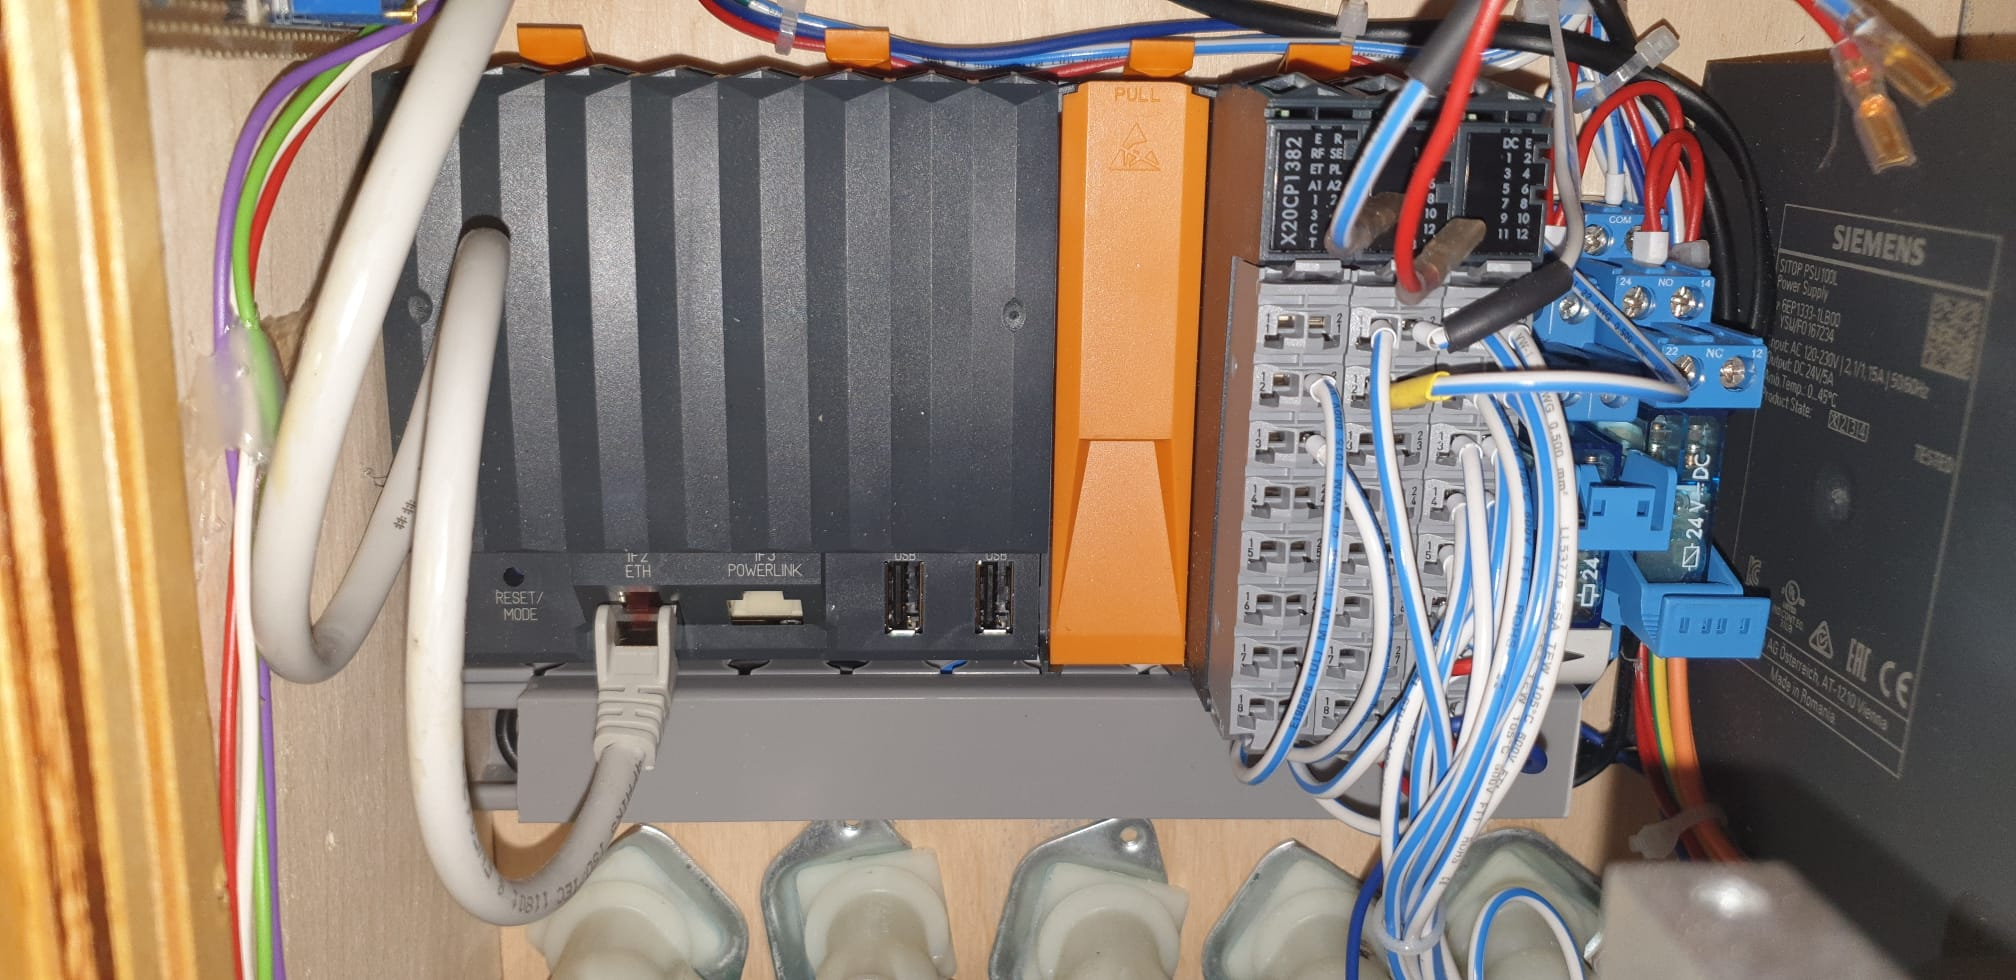
\includegraphics[width=1\textwidth]{IMG-20230913-WA0000}
		\centering
		\caption{Bild der SPS}
	\end{figure}
	\newpage
	
	\section{Auswahl des HMI}
	Auswahl: Power Panel 6PPT30 der Firma B\&R
	Als HMI oder Touchscreen hat sich das Power Panel 6PPT30 ergeben. Diese war in der Werkstatt vorhanden und ist vom selben Hersteller der Steuerung(B\&R). Da beide Geräte Steuerung und HMI vom selben Hersteller sind, gab es keine Kompatibilitätsprobleme.\\
	\begin{figure}[htb]
		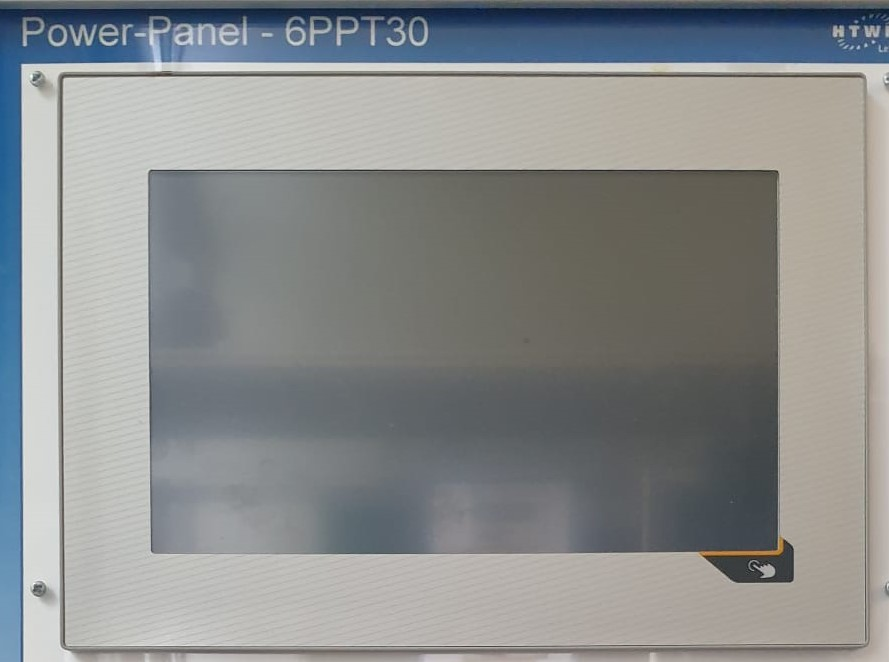
\includegraphics[width=0.9\textwidth]{IMG-20230913-WA0001}
		\centering
		\caption{Bild des Panels}
	\end{figure}
	\newpage
	\section{Auswahl der Antriebstechnik}
	Auswahl: Pumpenmotor 24 V   und DC-Motor 24 V 
	Für die Antriebstechnik wurden 2 Motoren benötigt, zum einen zum Befördern der Flüssigkeiten mit Druckluft und zum anderen zum Fördern des Eises. Wichtige technische Eigenschaften sind die Leistung und Anschlussmöglichkeit mit 24 V DC. Kühlung wird nicht benötigt, weil die Motoren nur bei Förderung eingesetzt werden und somit nicht lang genug eingesetzt werden, um zu überhitzen. Hierbei wurden Motoren benutzt, die schon im Lager vorhanden sind. 
	\subsection{Pumpenmotor 24 V}
	Es wurde ein Motor der Fa. KNF Neuberger verwendet mit dem Typenschild PJ 3616-06. Der Motor wird mit 24 V DC betrieben, hat eine Speisestrom von 1,1 A und eine Leistung bei Dauerbetrieb von 27,6 W. Ähnliche Motoren eignen sich auch für diese Aufgabe. Wichtigste Eigenschaft ist das der Motor mit 24 V DC betrieben wird!\\
	\begin{figure}[htb]
		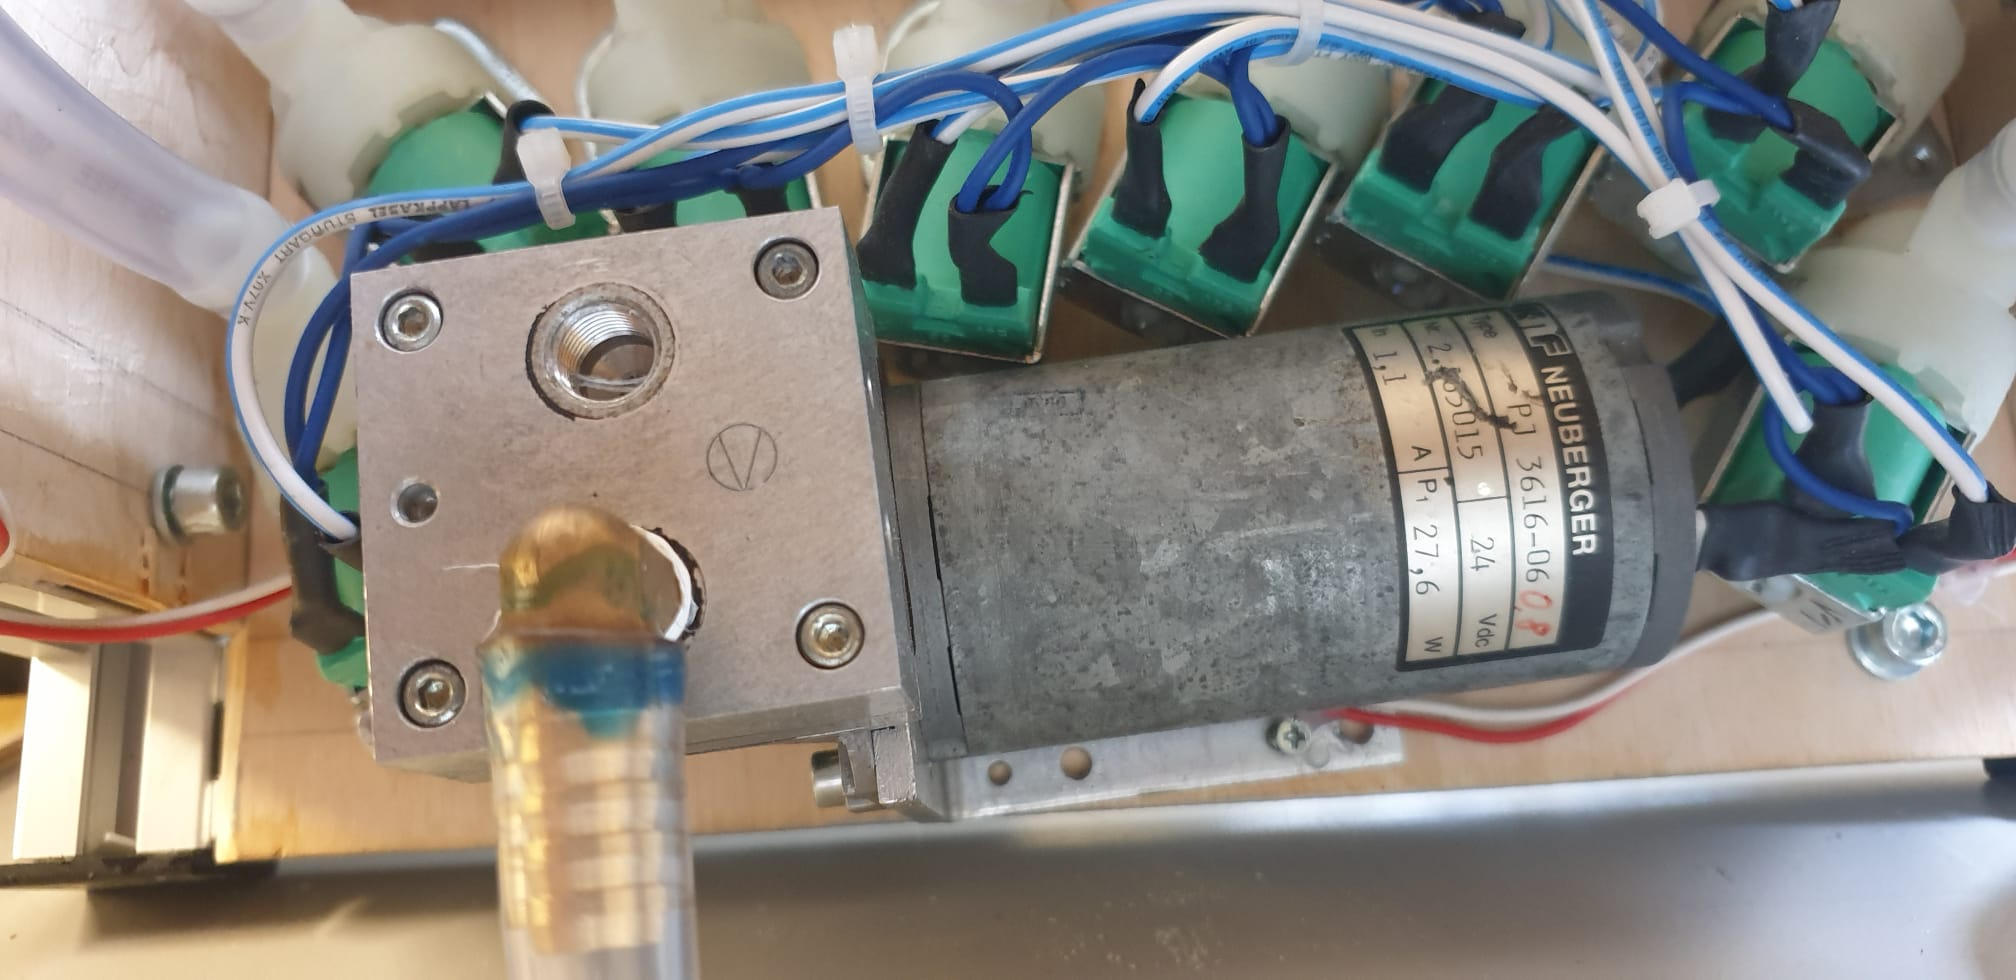
\includegraphics[width=1\textwidth]{Pumpenmotor}
		\centering
		\caption{Pumpenmotor}
	\end{figure} 
	\subsection{DC Motor 24 V mit Planetengetriebe Serie 38/1 S}
	Genutzt wird ein Motor mit Planetengetriebe der Fa. FAULHABER, welcher ebenso im Lager schon vohanden war. Wichtig ist hier ebenso das der Motor mit 24 V DC betrieben wird und eine Dauerdrehmoment bis 10 Nm leisten kann.\\
	\begin{figure}[htb]
		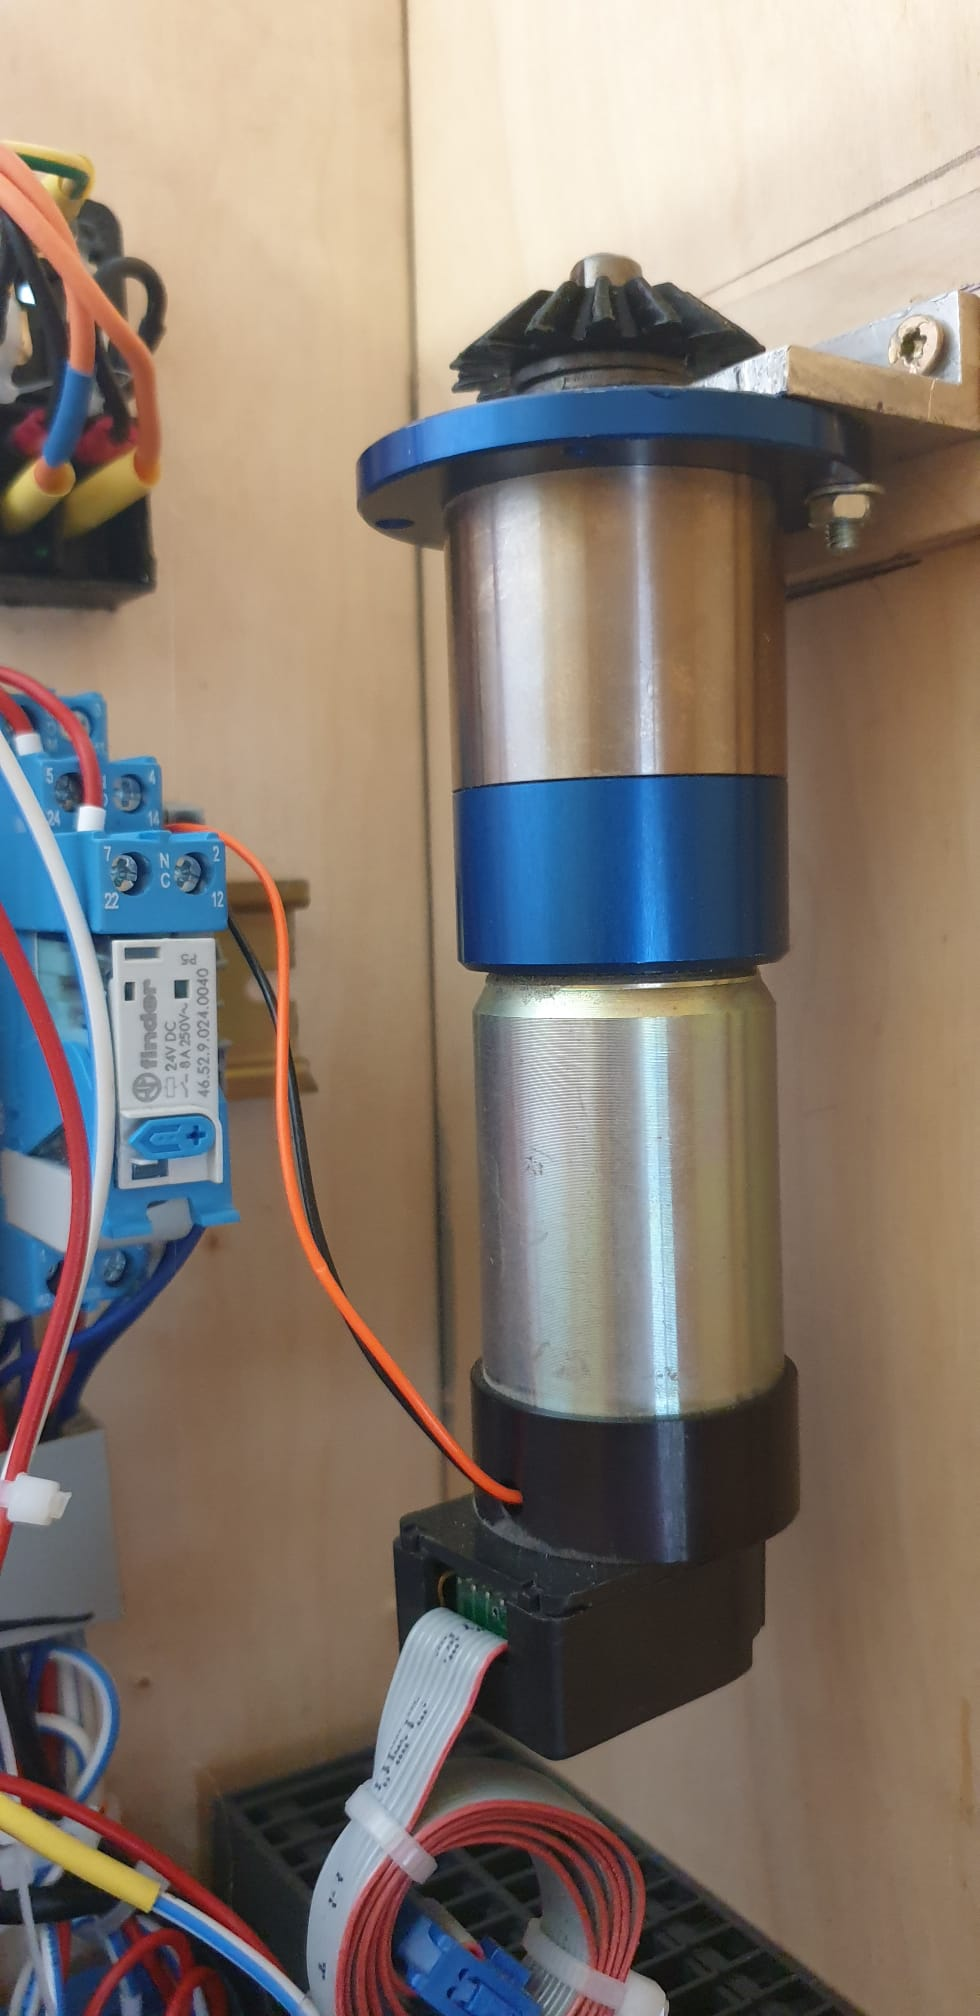
\includegraphics[width=0.2\textwidth]{Eismotor}
		\centering
		\caption{Eismotor}
	\end{figure} 
	\section{Auswahl des Feldbus}
	Auswahl: Ethernet\\
	\begin{figure}[htb]
		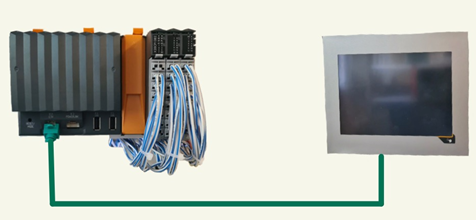
\includegraphics[width=1\textwidth]{Ethernet}
		\centering
		\caption{Ethernet}
	\end{figure}
	Wir nutzten 10/100 Base-T Ethernet inklusive einem im Bildschirm verbauten Switch, um die Komponenten SPS und Power-Panel zu verbinden. Für unsere Anwendung nutzten wir die 100-Mbit/s Variante. 
	Wir nutzten ein CAT 5e 100-Mbit/s-Ethernet Twisted Pair Kupferkabel mit einer Länge von 2 Metern. Dieses ist nach Verkabelungsart TIA-568A/B verkabelt. 
	Vorteile sind, dass der Bildschirm bis zu 100 m von der Cocktail-Maschine betrieben werden kann ohne Mehraufwand (Verstärker). CAT ist rückwärts kompatibel, es ist ein zuverlässiges und erprobtes System. 
	Ethernet hat eine einfache industrietaugliche Infrastruktur mit den CAT-Kabeln sowie den 8P8C-Modularstecker und -Buchsen (werden meist mit RJ-45 genannt). Man hat freie Wahl der Netzwerktopologien (Baum, Mesh, Ring, Stern).
	Im Allgemeinen gibt es keine Lizenzierungen.
	Ethernet entspricht den Normen TIA-568A/B (Standard für die Kontaktierung), IEEE-Norm 802.3 / 802.12 / 802.1Q, ISO/DIS 8802/3 (Ethernet-Standard), ISO/IEC 11801.
	Es gibt jedoch Technologien wie Universal Plug and Play (UPnP) oder Zero Configuration Networking (Zeroconf), die die Einrichtung von Netzwerkgeräten vereinfachen und automatische Konfigurationen ermöglichen. 
	Zusammengefasst kann man sagen, Ethernet ist einfach und schnell mit wenig Werkzeugen installiert. Einfach zu planen und die Kosten der Komponenten sind im Gegensatz zu anderen Feldbus-Systemen nicht kostenintensiv. \\
	
	\section{Auswahl der Feldgeräte}
	
	1. Lichtschranke E3Z R61 \\
	Der Sensor muss Betriebstemperaturen von 40 °C aushalten, zur Glaserkennung geeignet, Wasserdicht sein und eine
	Versorgungsspannung von 24 V DC haben. Diese Anforderungen werden alle erfüllt, da die Betriebstemperatur der Lichtschranke zwischen -25 °C und 55 °C liegt, die Empfindlichkeit einstellbar ist, die Lichtschranke eine Schutzart von IP67 und eine benötigte Versorgungsspannung von 24 V aufweist.\\
	
	\begin{figure}
		\begin{minipage}[b]{.4\linewidth}
			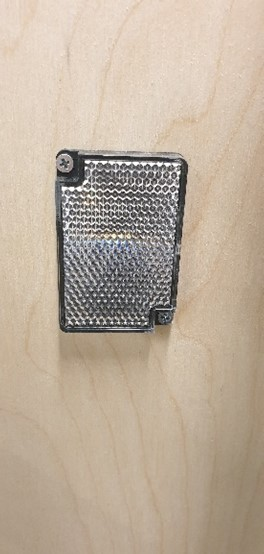
\includegraphics[width=0.9\textwidth]{Lichtschranke 1}
			\centering
			\caption{Reflektor}
		\end{minipage}
		\hspace{.1\linewidth}
		\begin{minipage}[b]{.4\linewidth}
			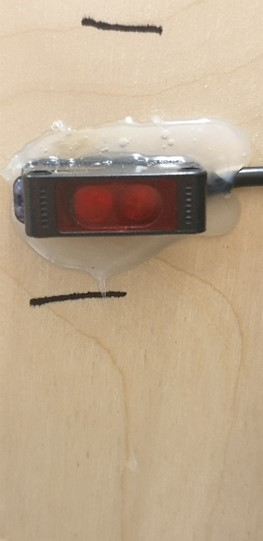
\includegraphics[width=0.9\textwidth]{Lichtschranke 2}
			\centering
			\caption{Sender und Empfänger}
		\end{minipage}
	\end{figure}
	\newpage
	2. Wägezelle Joy-it SEN-HX711-01 \\
	Die Wägezelle muss ebenfalls eine Betriebstemperatur von 40 °C aushalten und braucht einen Messbereich von ca. 1 kg. All diese Anforderungen erfüllt diese Wägezelle und ist zudem noch sehr günstig.\\
	
	\begin{figure}[htb]
		\includegraphics[width=0.8\textwidth]{Wägezelle}
		\centering
		\caption{Wägezelle}
	\end{figure}
	\newpage
	3. Messumformer ATO-LCTR-OA\\
	Die Anforderung, die an den Messumformer gestellt wird ist folgende: Eine Stromversorgung mit 24 V DC muss gewährleistet sein, Betriebstemperaturen im Bereich 40°C dürfen keine Probleme bereiten, eine Ausgabesignal von 4-20 mA oder 0 - 10 V müssen vorhanden sein und es darf nicht zu teuer sein. All diese Anforderungen erfüllt der Messumformer ohne Probleme. Der Messumformer kann im Bereich von 18 - 30 V DC betrieben werden, erfüllt auch im Bereich von 40°C ihre Aufgabe und bei einem Preis von 38,55€ für eine Einmalbeschaffung sehr preisgünstig.
	\begin{figure}[htb]
		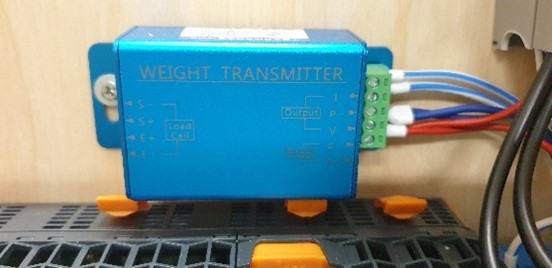
\includegraphics[width=0.8\textwidth]{Messumformer}
		\centering
		\caption{Messumformer}
	\end{figure}
	
	4. Ventil R Mini -510 der Hersteller RPE\\
	Für die Ventile gilt, dass diese lebensmittelecht sein müssen, Umgebungstemperaturen von 40°C keine Probleme machen, die Ventile mit 24 V DC angesprochen werden können und auch wirtschaftlich sein müssen. \\
	Das Ventil R Mini -510 besitzt Zulassungen, um als Ventil für Trinkwasser genutzt zu werden. Das Ventil darf laut Datenblatt in einer Umgebungstemperatur von 0 °C bis 60 °C betrieben werden. Das Magnetventil kann mit 24 V DC der SPS angesprochen werden.
	Da 8 Magnetventile benötigt werden, gab es einen Mengenrabatt. Wodurch ein Ventil 18,28 € kostet, was einen Rabatt von 10\% ausmacht. Natürlich könnten auch billigere Varianten genommen werden, wodurch aber keine Lebensmittelechtheit garantiert ist.
	\begin{figure}[htb]
		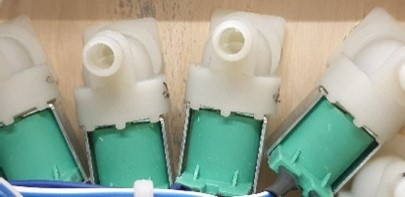
\includegraphics[width=0.8\textwidth]{Ventil}
		\centering
		\caption{Ventil}
	\end{figure}
	
	5. Koppel-Relais 49.52.9.024.0050 der Firma Finder\\
	Das Relais muss mit 24 V DC ansprechbar sein, eine Umgebungstemperatur von 40 °C aushalten, einen zugelassenen  Schaltstrom von 400 mA schalten können und Montierung auf einer Hutschiene muss möglich sein.
	Das Relais erfüllt diese Bedingungen ohne Probleme. Das Relais kann mit 24 V DC der SPS angesprochen werden. Die Betriebstemperaturen liegen bei -40 °C bis 70 °C. Der maximale Schaltstrom liegt bei 8 A. Der Baustein kann auf eine Hutschiene montiert werden.
	\begin{figure}[htb]
		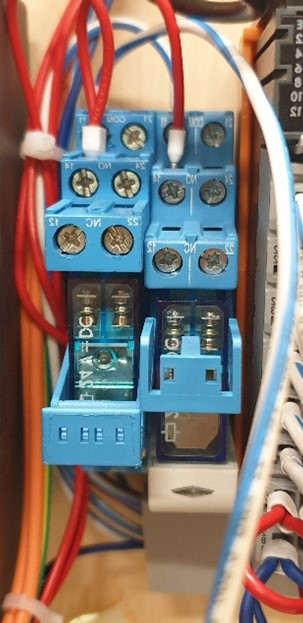
\includegraphics[width=0.5\textwidth]{Relais}
		\centering
		\caption{Relais}
	\end{figure}

	\section{Auswahl der Spannungsversorgung}
	Auswahl: Siemens SITOP PSU100L 24 V/5 A Hutschienen-Netzteil\\
	Die wichtigste Eigenschaft der Spannungsversorgung ist, dass sie genug Leistung für alle Systeme bereitstellen muss und für das gedachte und reale Umfeld genutzt werden kann. Dafür reicht das gewählte Netzteil völlig aus. Zudem war dieses Netzteil auch schon im Lager, wodurch teure Einkäufe nicht getätigt werden mussten. 
	
	\begin{figure}
		\begin{minipage}[b]{.4\linewidth}
			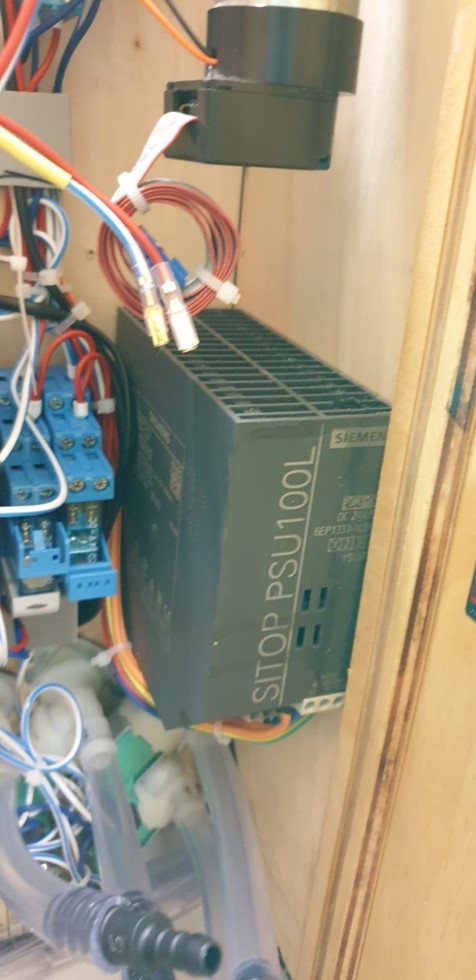
\includegraphics[width=0.9\textwidth]{Netzteil 1}
			\centering
			\caption{Eingebautes Netzteil}
		\end{minipage}
		\hspace{.1\linewidth}
		\begin{minipage}[b]{.4\linewidth}
			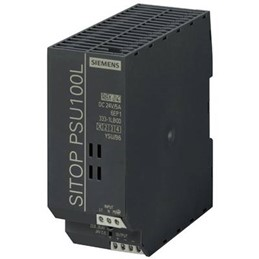
\includegraphics[width=0.9\textwidth]{Netzteil 2}
			\centering
			\caption{Netzteil außerhalb}
		\end{minipage}
	\end{figure}	
	
	\chapter{Gehäuseaufbau}
	
	Das Grundgehäuse gehört zu den Hauptbestandteilen der Cocktailmaschine. Es muss zum einen von außen attraktiv für den Anwender wirken, zum anderen muss es genügend Platz für die Technik innerhalb bieten und darf keine Abläufe behindern. Außerdem trägt das Gehäuse das gesamte Gerät. Daher ist es wichtig, sich für stabile Materialien zu entscheiden, die das Eigengewicht der Maschine tragen können.
	Wir haben uns für eine schlichte Grundform entschieden, eine Art Quader. Dies erinnert auch an handelsübliche ähnliche Geräte, wie z.B. Kaffeeautomaten. Um möglichst viel Stabilität zu erreichen, dienen Profilschienen aus Aluminium als Grundskelett. Um alle Profilschienen miteinander zu verbinden, haben wir uns den Aufbau des Querschnitts zum Vorteil gemacht. Profilschienen sind nicht komplett massiv, da sie auch mit einigen Hohlräumen sehr stabil sind und zudem der Materialverbrauch geringer ist. Daher verläuft durch die Mitte des Querschnitts ein rundes Loch, in welches wir ein Gewinde gefräst haben. Durch die anderen Profilschienen wurde von außen ein Loch auf gleicher Höhe gebohrt, sodass man alle Profilschienen mit Schrauben befestigen kann. Eine besonders wichtige Profilschine haben wir vorne auf ungefähr halber Höhe platziert. Diese dient zum befestigen der Wägezelle, auf der der Cocktailbecher platziert wird.
	Damit die Cocktailmaschine Gestalt annimmt, braucht es natürlich mehr als das Grundskelett. Daher war die nächste Aufgabe, Wände in passender Größe hinzuzufügen. Dabei haben wir uns für Holzplatten entschieden. Grund dafür ist, dass solches Holz nicht zu teuer ist, man leicht Löcher und Öffnungen hineinsägen kann, es stabil genug ist, um an ihm mögliche elektrische Geräte zu befestigen und es eine gute Struktur für spätere Gestaltung bietet. 
	Im letzten Teil des Gehäuses wurde an einer Trennwand gearbeitet. Sie dient dafür, dass zum einen der Anwender die Elektronik im hinteren Teil nicht sieht, zum anderen schützt die Trennwand die empfindliche Elektronik vor Flüssigkeiten, die eventuell daneben laufen. Auch hier haben wir uns für eine Holzwand entschieden, die mit einer Schiebekonstruktion heraus- und hineingeschoben werden kann. Damit das Holz nicht durch die Flüssigkeiten beschädigt wird, wurde der gesamte vordere Innenraum und die Trennwand mit einem Lack isoliert. Das Fertige Gehäuse sehen sie in der Abbildung 5.1\\
	
	\begin{figure}[htb]
		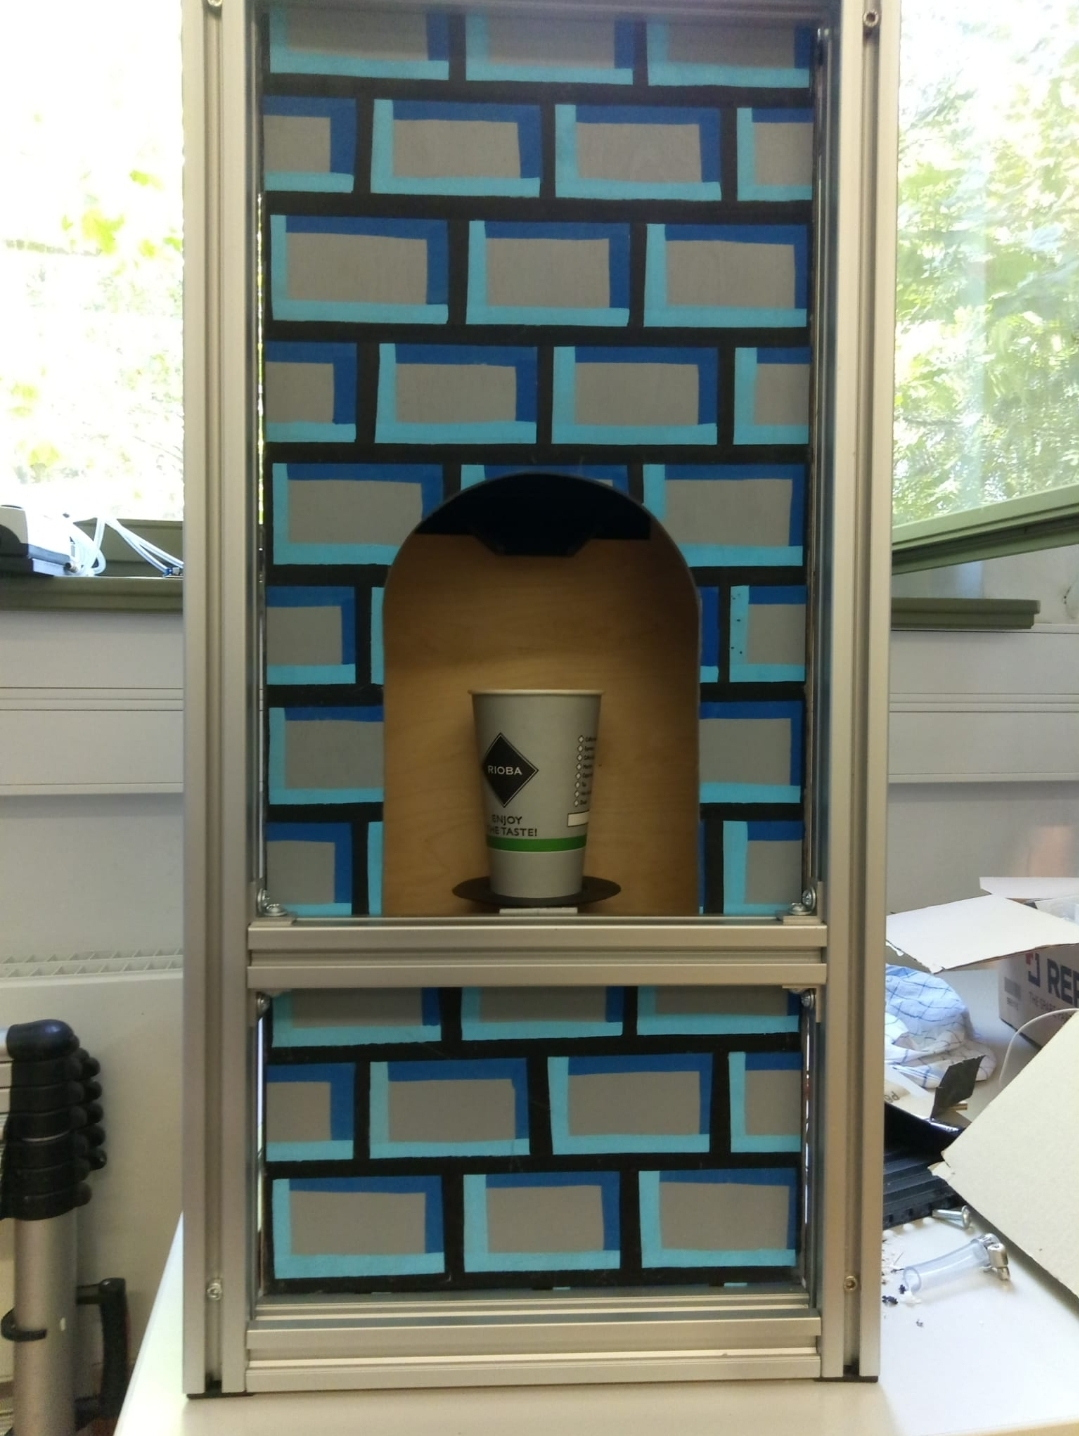
\includegraphics[width=0.9\textwidth]{Abb.11_fertige_Cocktailmaschine}
		\centering
		\caption{Cocktailmaschine}
	\end{figure}

	\chapter{Verkabelung}
	Die Verkabelung von elektrischen Systemen ist ein grundlegendes und entscheidendes Element in nahezu jeder modernen Anwendung von Elektrizität und auch hier ist das der Fall. 
	Mithilfe von Stromlaufplänen lässt sich die Verkabelung auch leicht realisieren. 
	Wir fangen hier bei der Verkabelung der SPS an, die Stromversorgung, gehen dann auf die Verkabelung der Pneumatik ein und enden mit der Verkabelung der LEDs. 
	Grundsätzlich wurden zur Verkabelung Kupferkabel mit einer Querschnittsfläche von 0,75 mm² genutzt. Wenn möglich wurden immer Aderendhülsen genutzt und wenn nicht wurde gelötet.
	
	Aus dem Handbuch der SPS kann man die Anschlussbelegung erkennen.
	
	\begin{figure}[htb]
		
\includegraphics[width=1\textwidth]{H1}
		\centering
		\caption{Anschlussbelegung des integrierten I/O-Steckplatzes X1}
	\end{figure}
	
	Um Überkopplungen zu vermeiden, sollte jede Signalleitung der schnellen digitalen Eingänge einzeln geschirmt
	werden. Die maximale Leitungslänge beträgt 20 m.
	
	\begin{figure}[htb]
		
\includegraphics[width=1\textwidth]{H2}
		\centering
		\caption{Anschlussbelegung des integrierten I/O-Steckplatzes X2}
	\end{figure}
	\newpage
	\begin{figure}[htb]
		
\includegraphics[width=1\textwidth]{H3}
		\centering
		\caption{Anschlussbelegung des integrierten I/O-Steckplatzes X3}
	\end{figure}
	Wir fangen hier bei dem Steckplatz X1 an. 
	Es werden die Anschlüsse AI + 2 U und AI – 2 U/I genutzt. Mit diesen beiden Anschlüssen ist die Wägezelle verbunden. Natürlich kann man auch AI +1 U und und AI – 1 U/I nutzen, jedoch hatte unsere genutzt SPS ein technisches Problem, wodurch diese nicht genutzt werden konnten. Wir konnten jedoch auf die danebenliegenden Analogen Eingänge ausweichen. 	
	Der Steckplatz X2 wird für Digitale Eingänge genutzt. DI 1 wird für die Lichtschranke genutzt, DI 2 für den Endlagenschalter (schwarz) vom Eismotor und DI 3 für den Enlagenschalter (gelb) vom Eismotor. 	
	Der Steckplatz X3 wird genutzt für Digitale Ausgänge und für die Spannungsversorgung von SPS und I/O-Systeme. DO 1-8 werden für Ventile genutzt. Also DO 1 für Ventil 1 etc. pp. DO 9 wird genutzt zum Schalten der Pumpe, DO 10 für das Schalten des Eismotors genutzt, DO 11 für grüne LEDs und DO 12 für rote LEDs Die restlichen Steckplätze werden zur Spannungsversorgung genutzt +24 V SPS und GND sowie +24 V I/O und wieder GND. 
	Das wird hier ersichtlich: \\
	
	\begin{figure}[htb]
		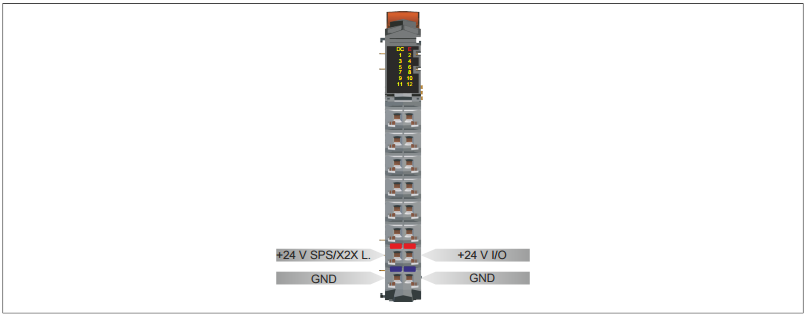
\includegraphics[width=1\textwidth]{H4}
		\centering
		\caption{Anschlussbelegung für die Stromversorgung}
	\end{figure}
	\newpage
	Als Stromlaufplan für die Eingänge ergibt sich dann: \\
	\begin{figure}[htb]
		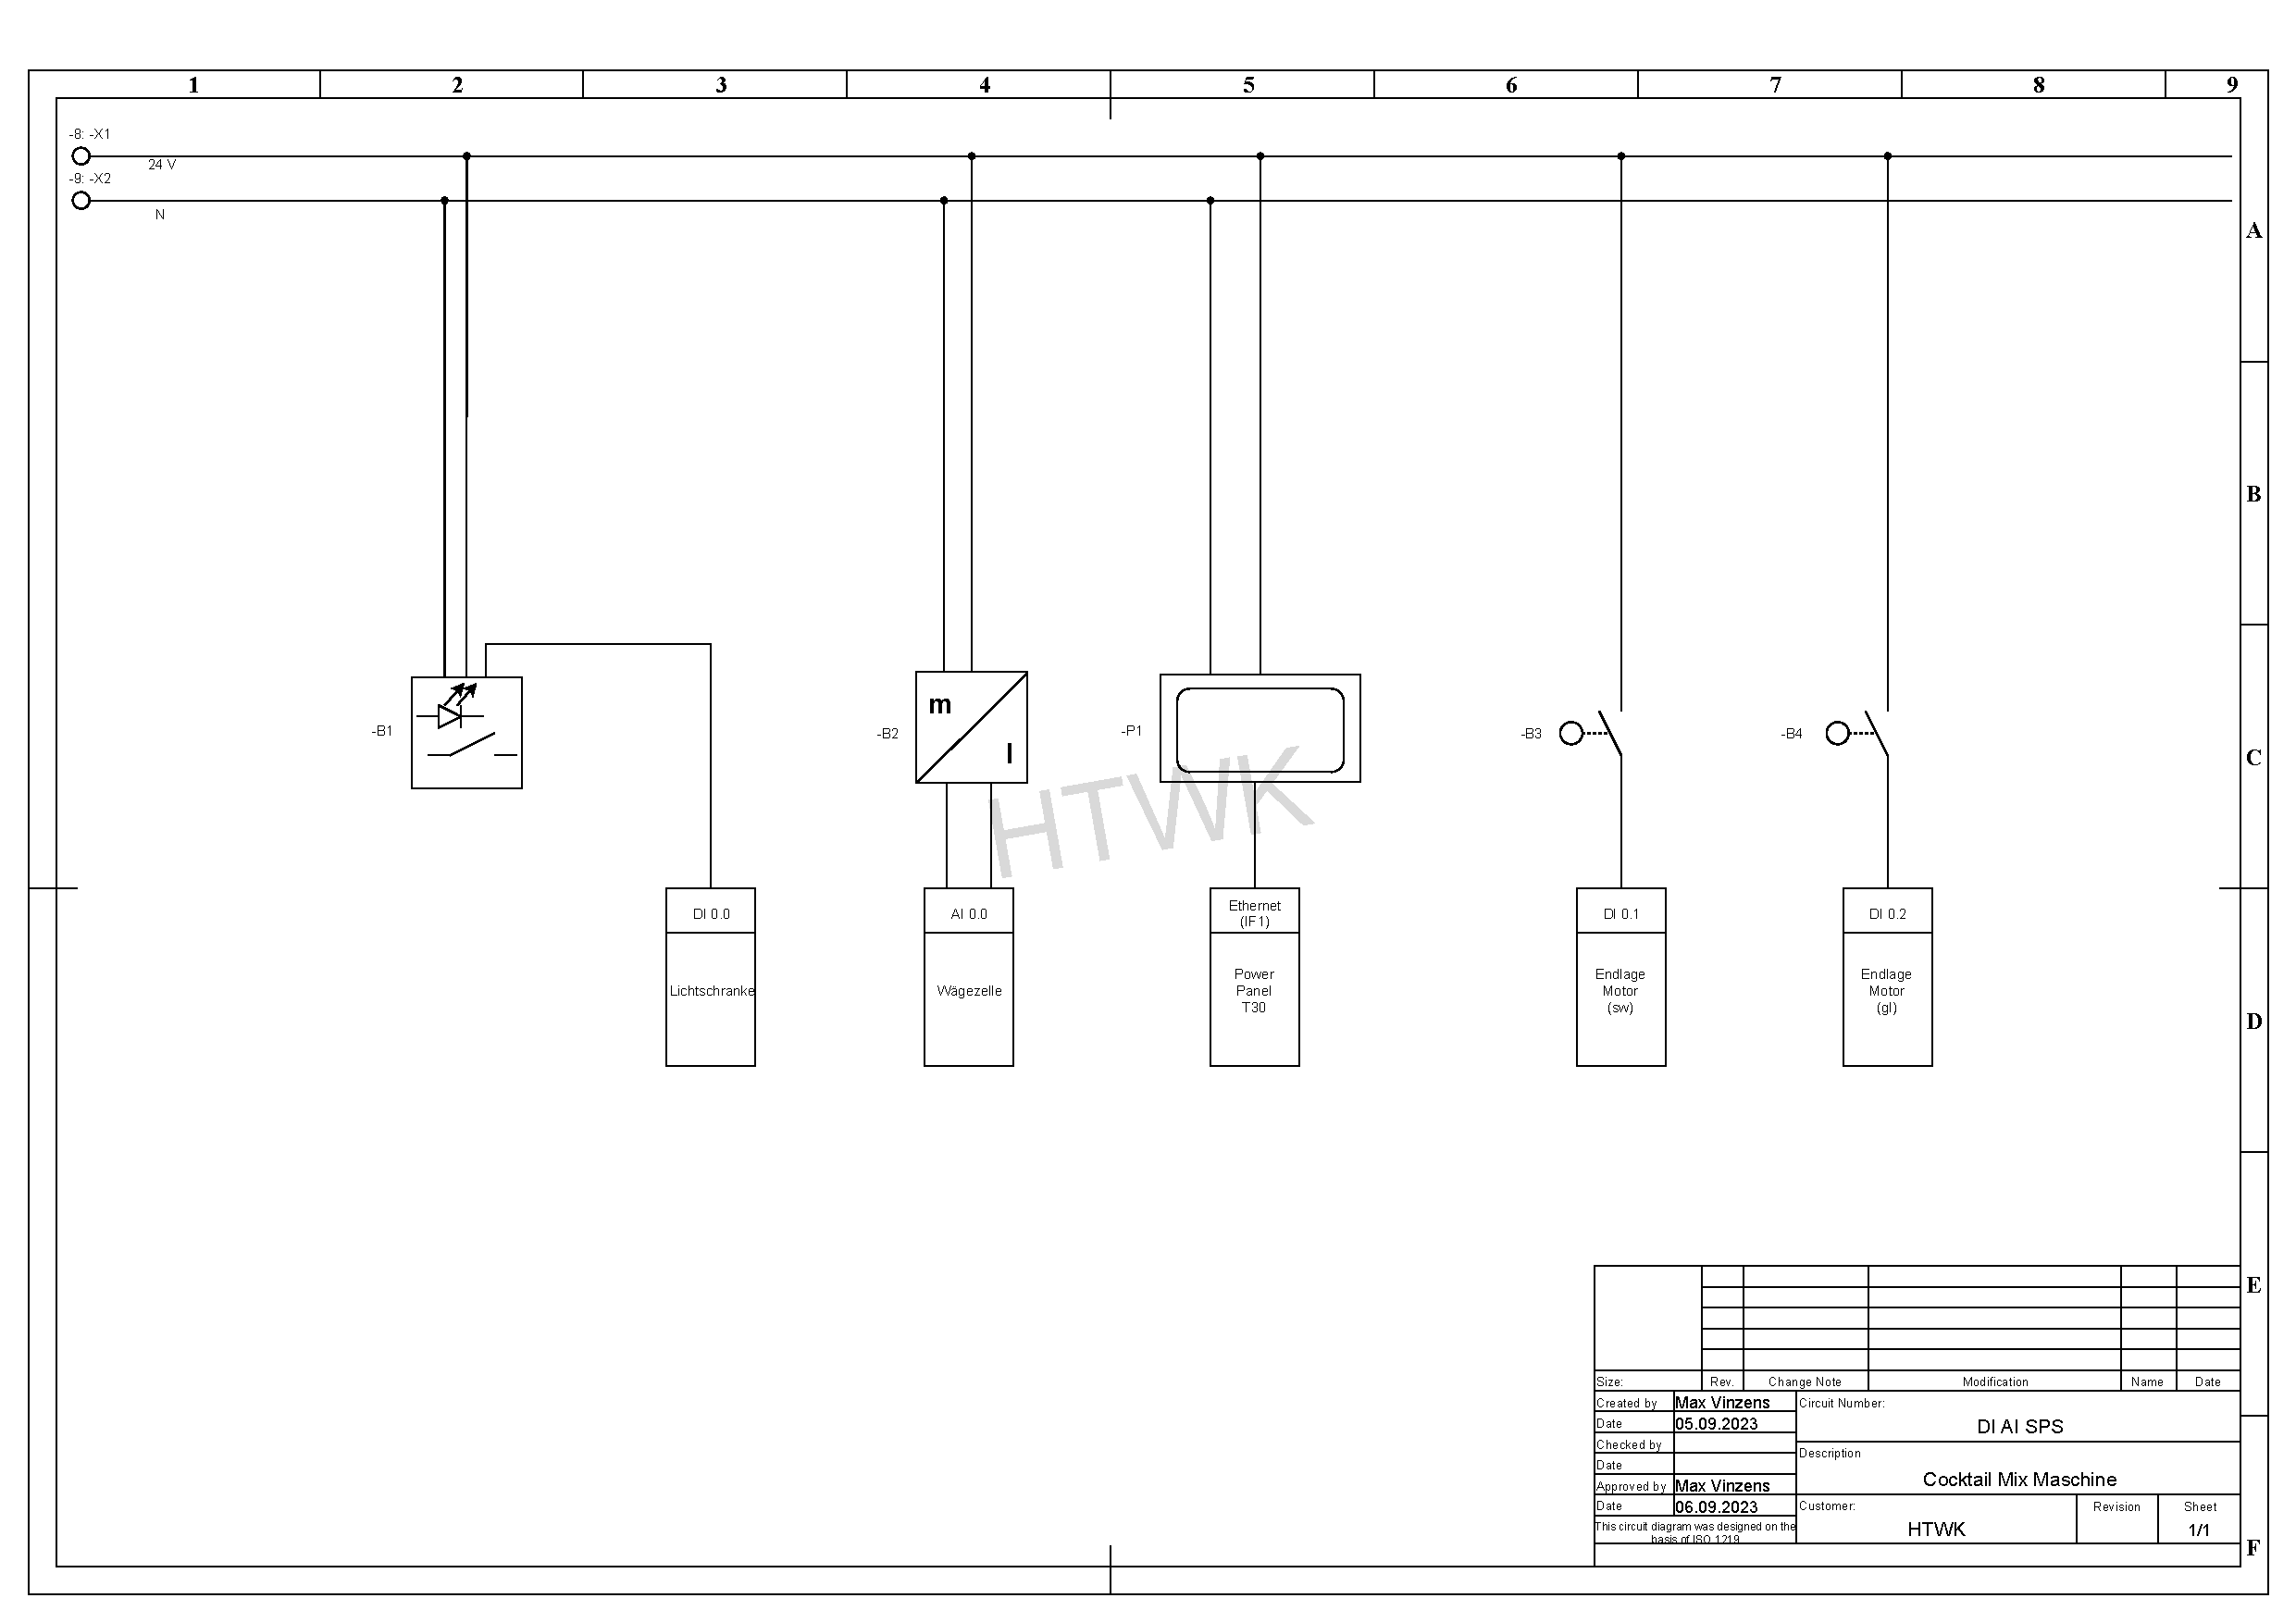
\includegraphics[width=0.75\textwidth]{DI AI (V2).pdf}
		\centering
		\caption{Stromlaufplan Eingänge}
	\end{figure}
	\\Als Stromlaufplan für die Ausgänge, auch Pneumatik(Ventile und Pumpe) ergibt sich: \\
	\begin{figure}[htb]
		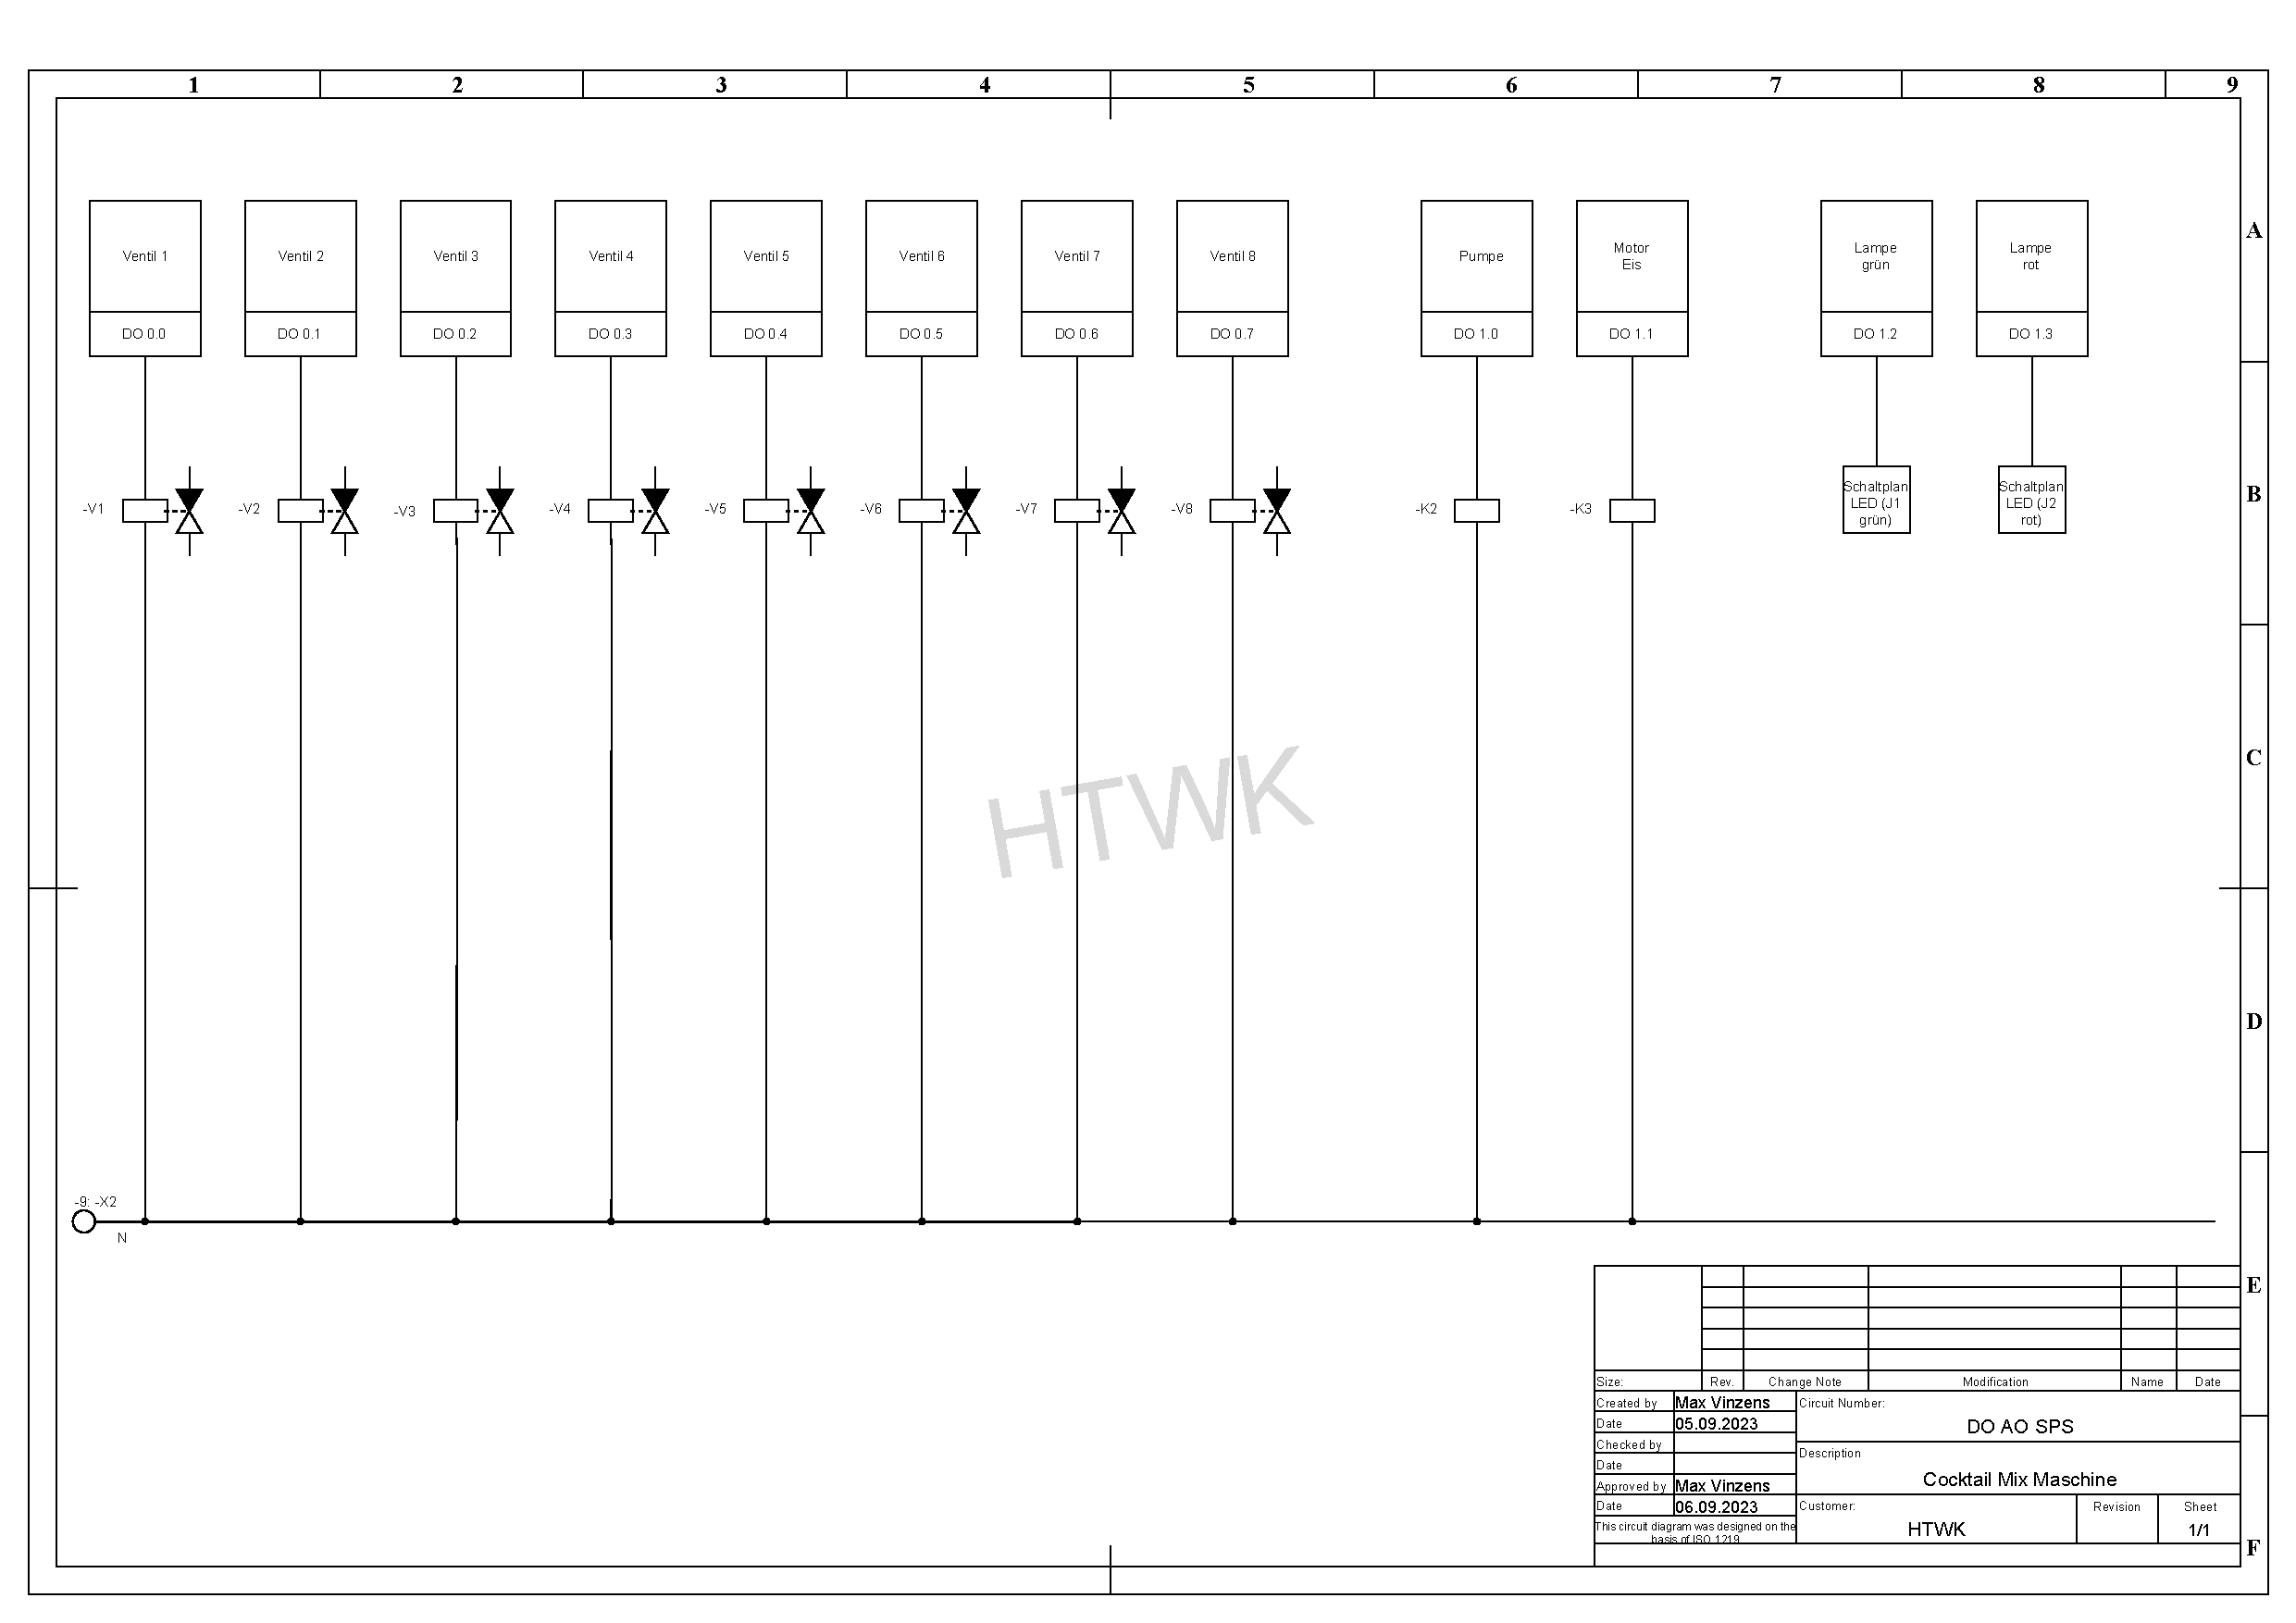
\includegraphics[width=0.75\textwidth]{DO AO SPS (V2).pdf}
		\centering
		\caption{Stromlaufplan Ausgänge}
	\end{figure}
	\newpage
	Die Stromversorgung wird über ein Netzteil von Siemens realisiert.\\ 
	\begin{figure}[htb]
		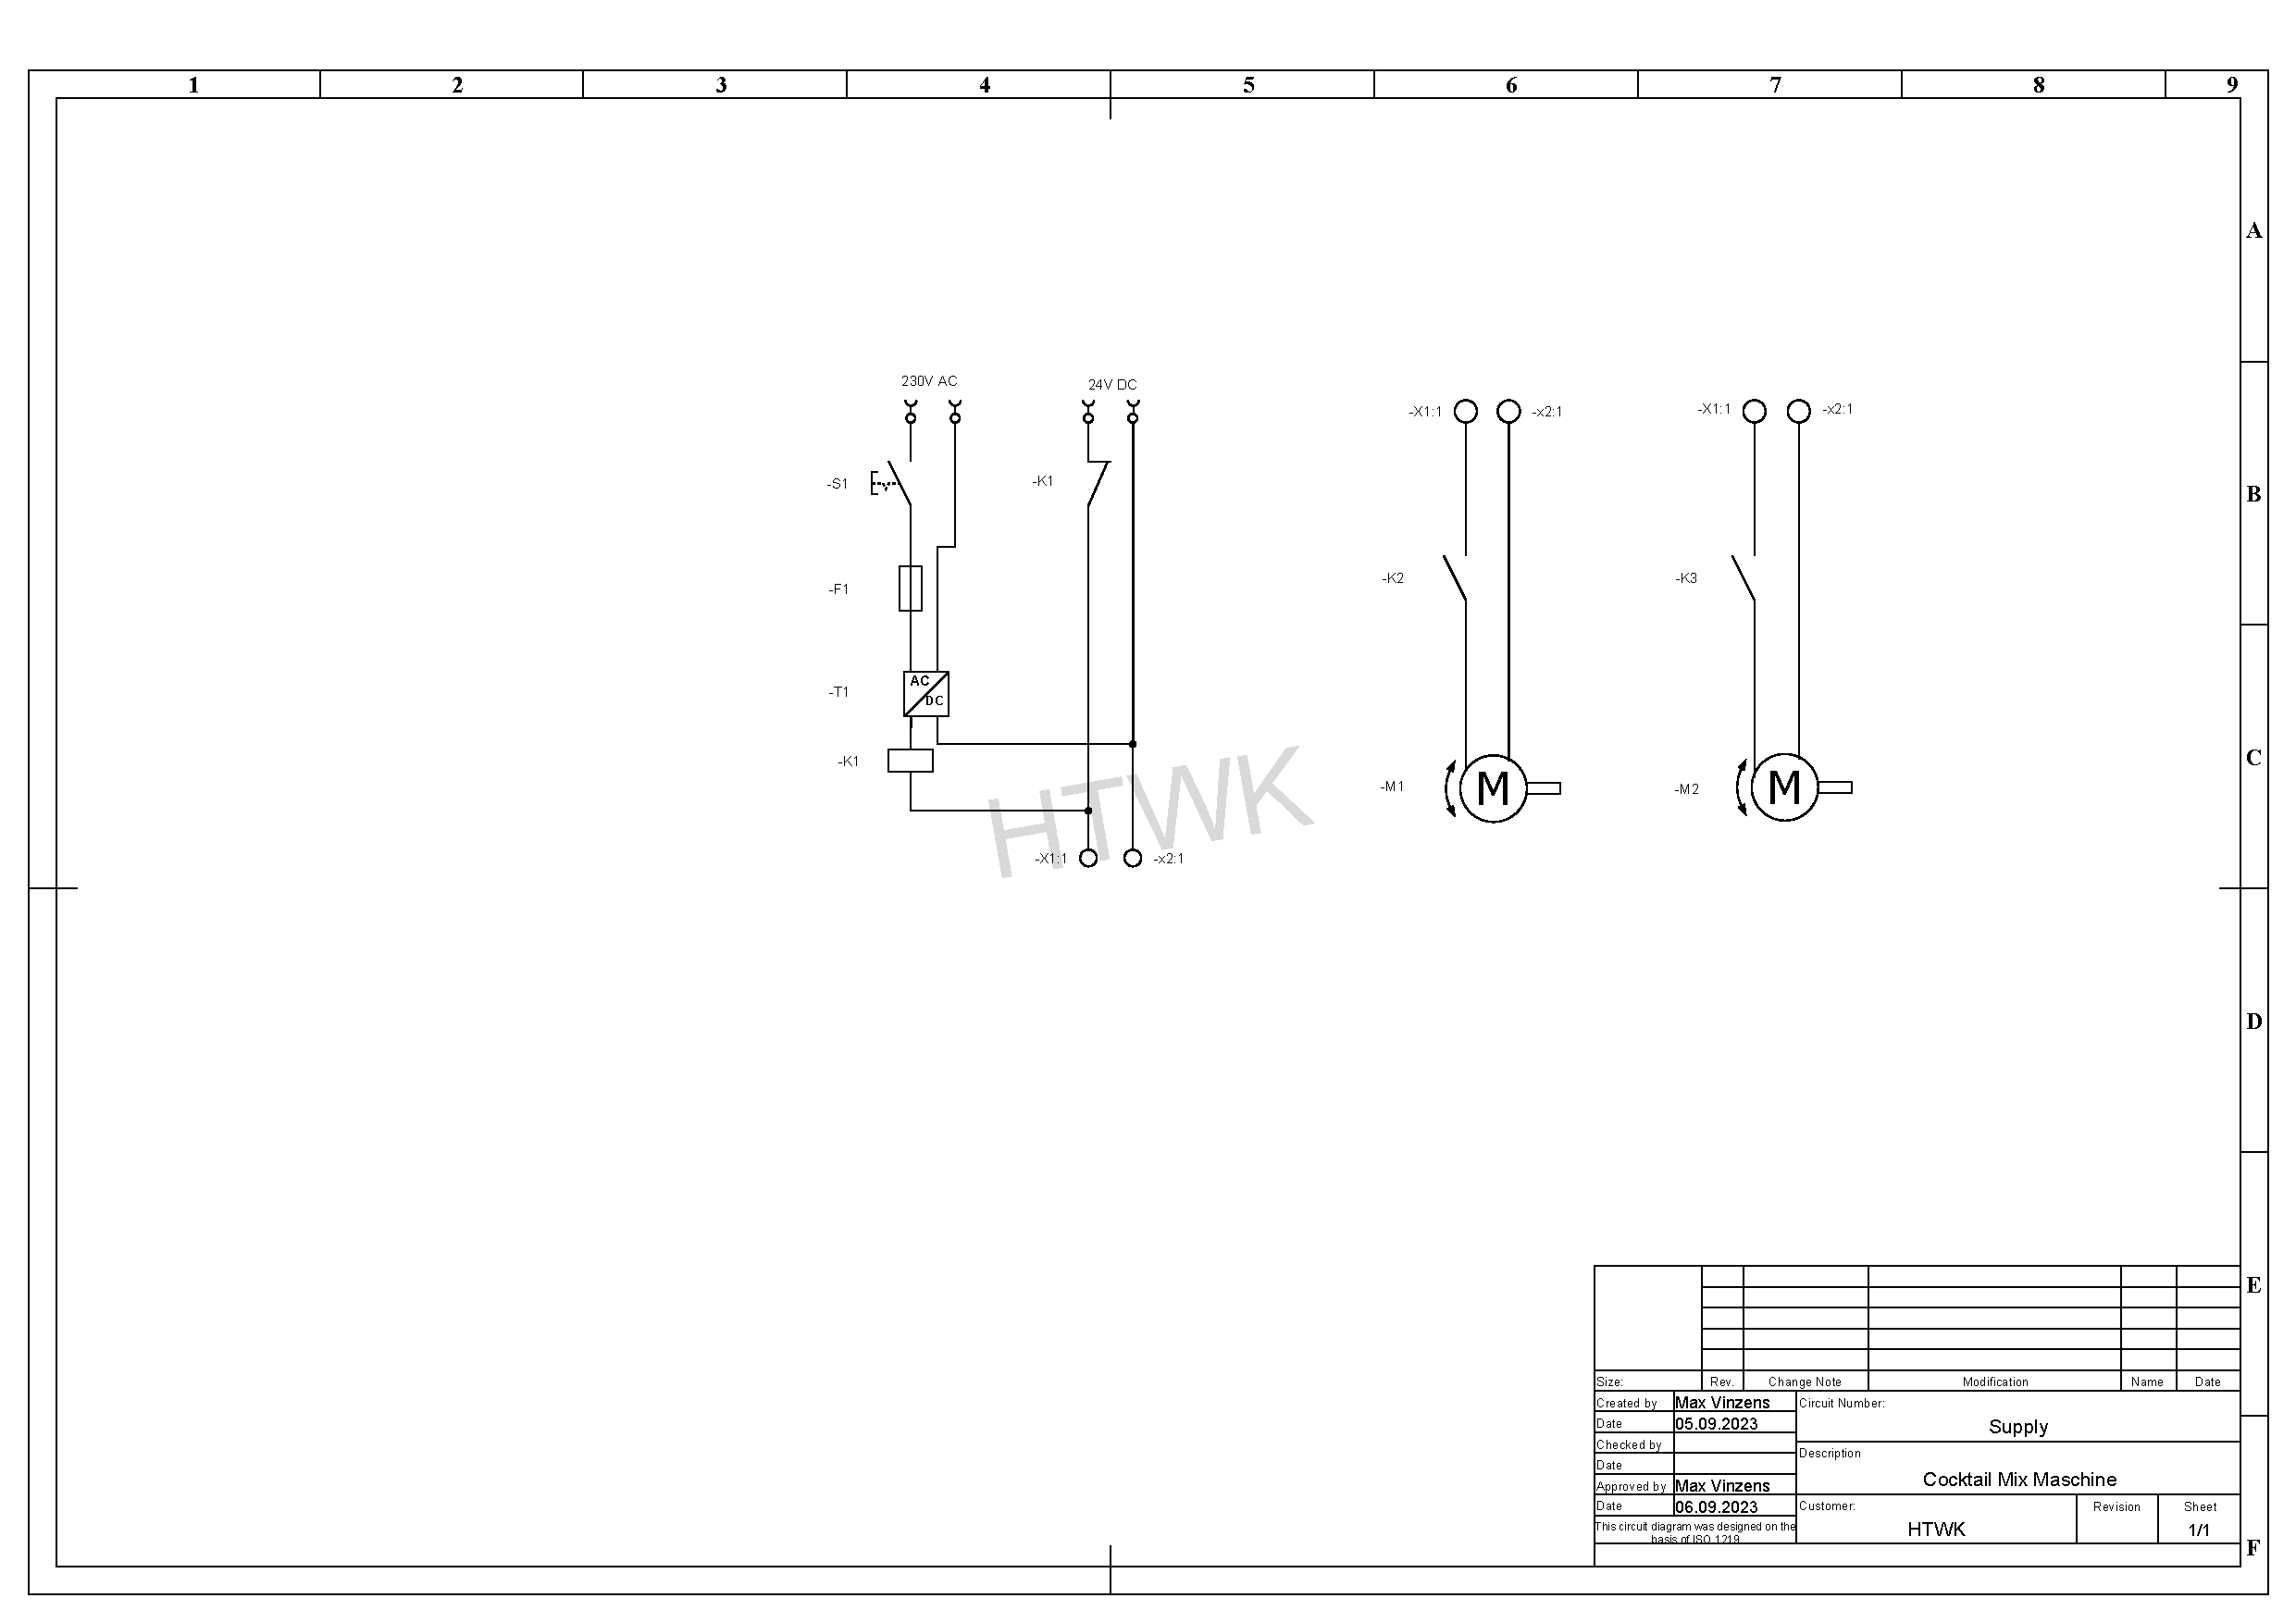
\includegraphics[width=0.75\textwidth]{Supply (V2) .pdf}
		\centering
		\caption{Stromversorgung}
	\end{figure}
	\\Die LEDs werden so verkabelt:\\
	\begin{figure}[htb]
		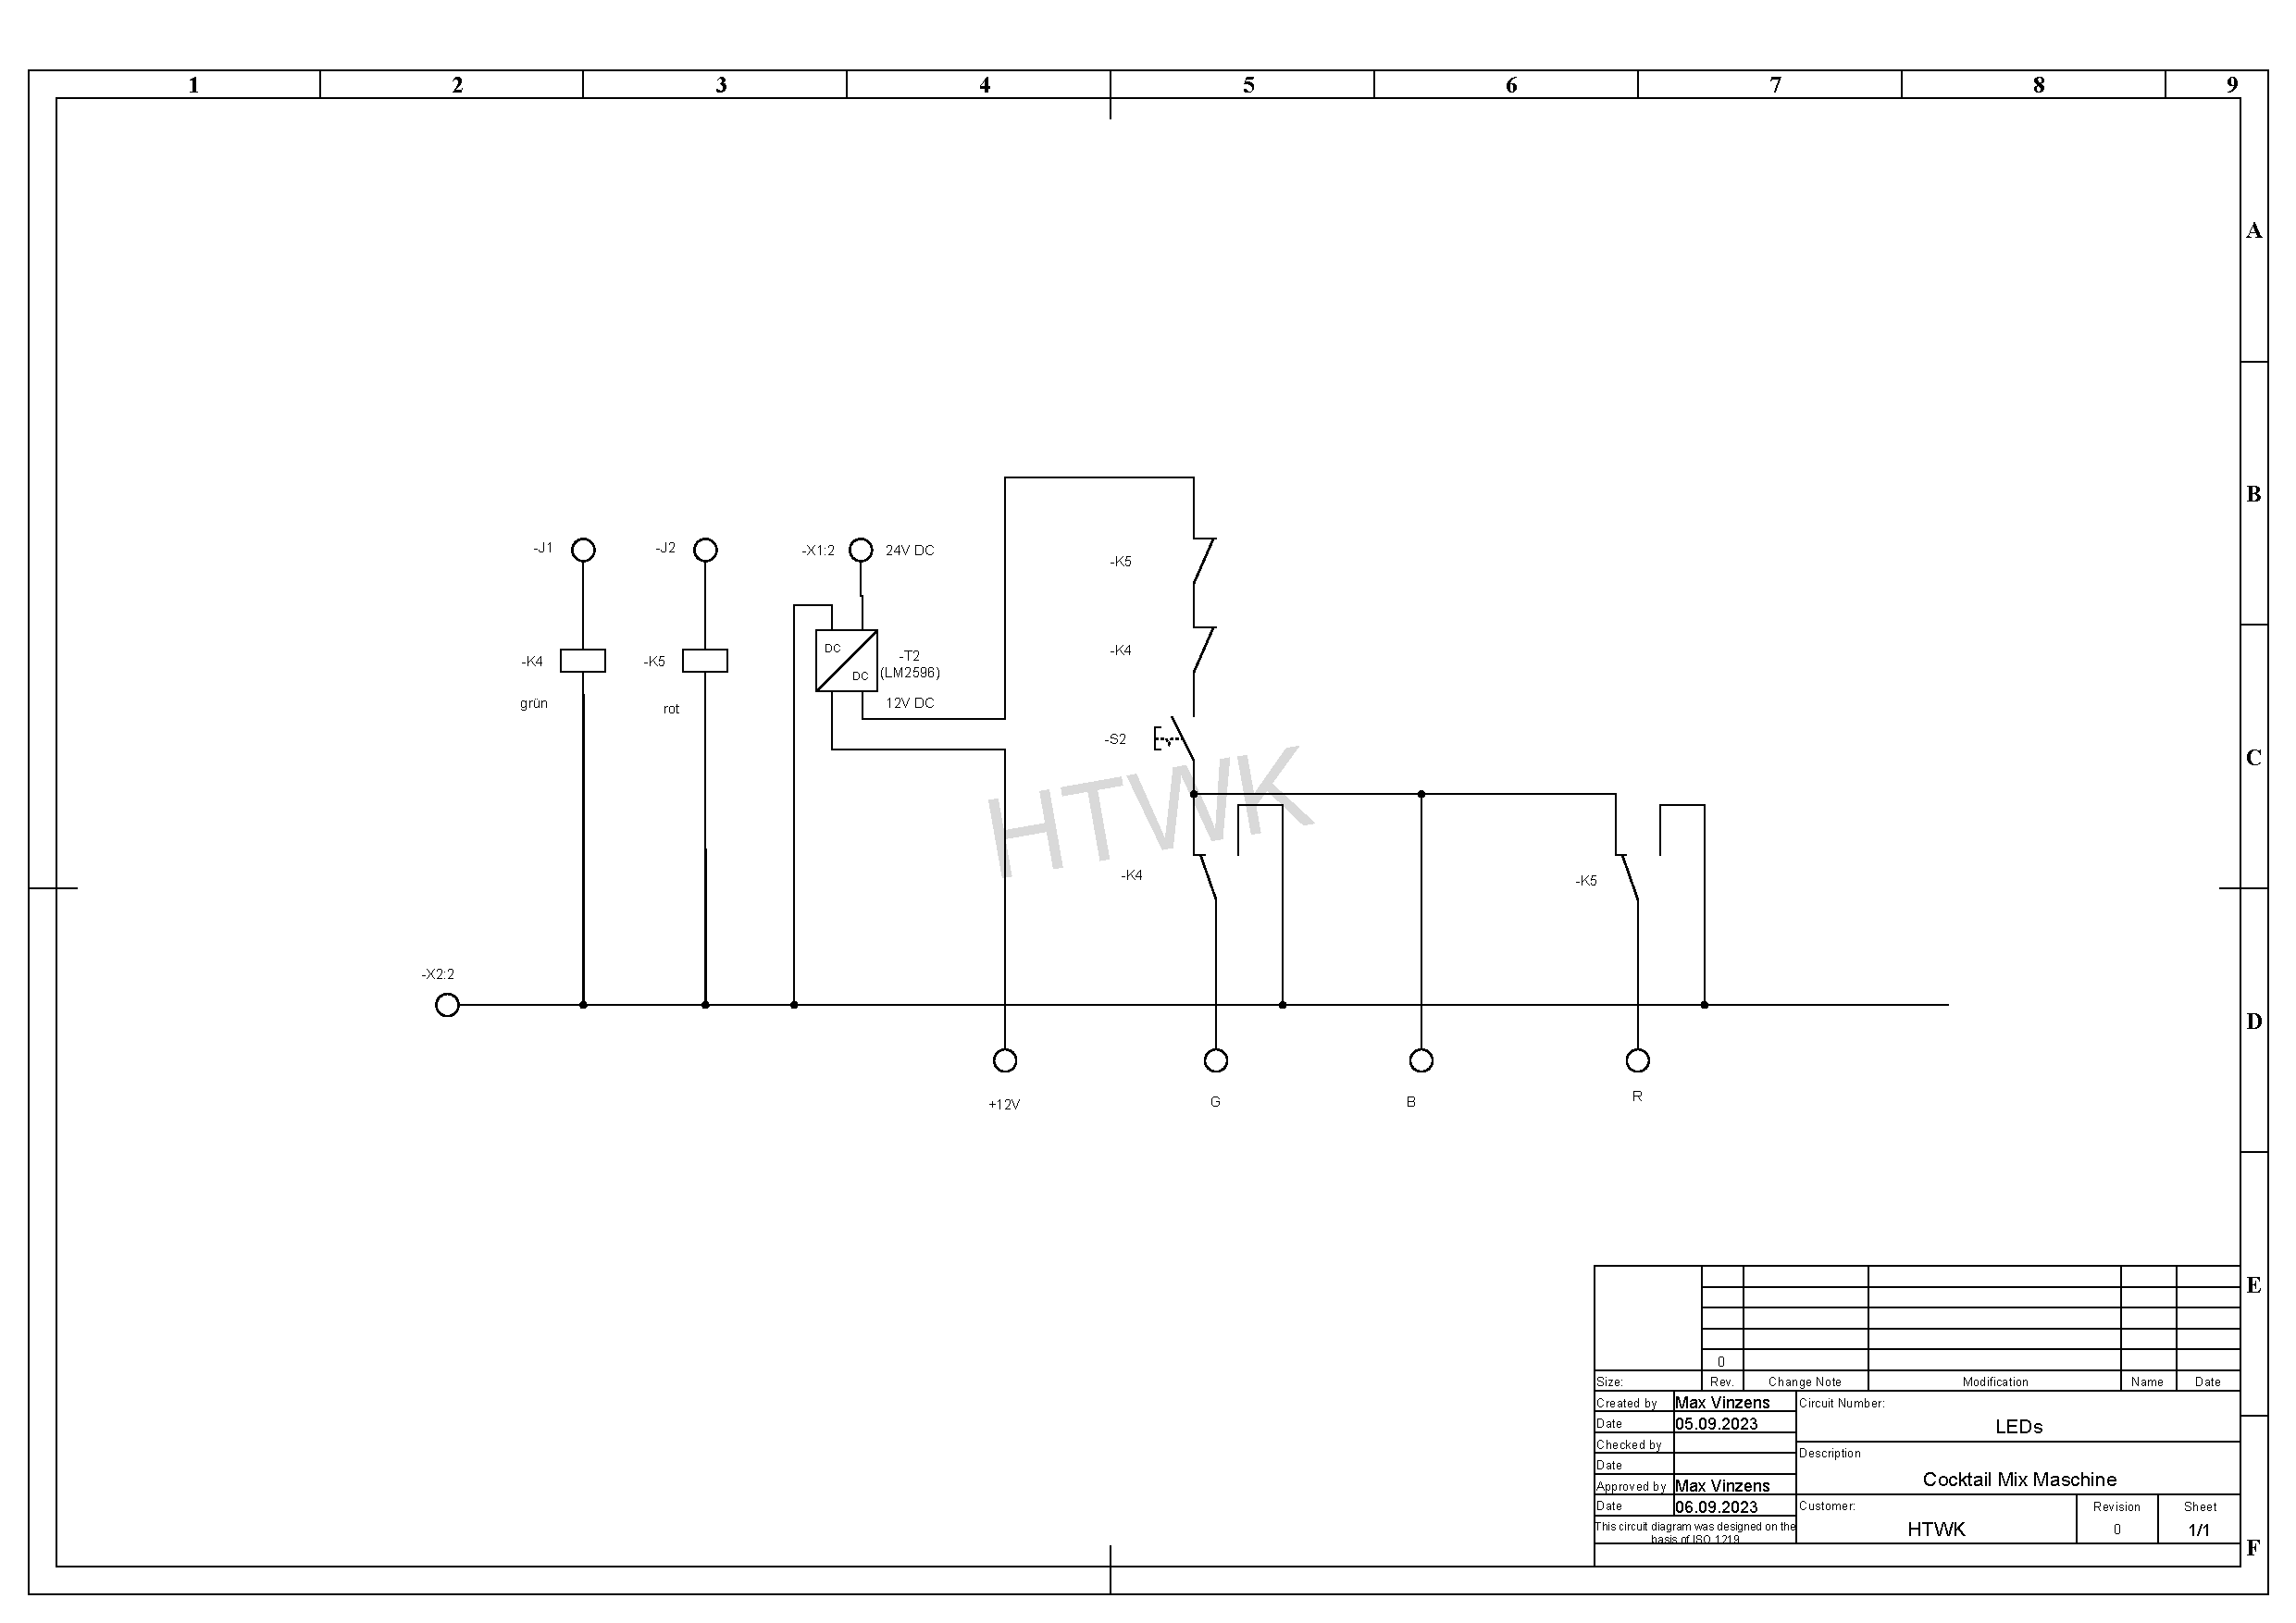
\includegraphics[width=0.75\textwidth]{LEDs (V2).pdf}
		\centering
		\caption{LEDs}
	\end{figure}
	\\Die LEDs werden mit 12 V versorgt, daher wird ein Spannungsregler, gekennzeichnet mit T2, benötigt. Es werden 2 Relais genutzt, für grün und rot, gekennzeichnet mit K4 und K5. Wenn die mit den Relais verbundenen LEDs nicht geschaltet werden von der SPS, dann entsteht ein kaltweißes Licht, weil alle LEDs an gehen.
	 
	\chapter{Verschlauchung}
	
	\section{Aufgabe}
	Wir haben acht Behälter mit unterschiedlichen Flüssigkeiten, dabei ist die Viskosität, Dichte, sowie
	die Sedimentbildung unterschiedlich. Hinzu kommt, dass die Behälter ca. 1 Meter unter der
	Cocktailmaschine stehen und die Flüssigkeiten ca. 1,50 Meter hoch gefördert werden muss.
	Dadurch das die Schläuche, Ventile und die Behälter mit dem Produkt (Lebensmittel) in Berührung
	kommen muss alles Lebensmittelecht sein. Das heißt, sie bestehen aus unbedenklichen Stoffen,
	haben keine Geruchsveränderung und haben keine Geschmacksverändern-Wirkung auf das
	Endprodukt. Die Schläuche sollten EU Nr.10 2011 geprüft sein.\\\\
	
	\section{Problemlösung}
	Am Anfang hatten wir drei verschiedene Lösungskonzepte.\\ \\
	1. In jedem Behälter wird eine Pumpe installiert.\\
	- Vorteil: einfach umzusetzen\\
	- Nachteil: acht Pumpen mit unseren Spezifikationen sind sehr kostenintensiv\\ \\
	2. Die Druckluft, die zum Behälter geht, wird mit einem Ventil gesteuert.\\
	- Vorteil: keine Lebensmittel echten Ventile sowie nur eine Pumpe für die Luft\\
	- Nachteil: schlecht zu steuern, da der Füllstand vom Behälterhöhe abhängen\\ \\
	3. Die Behälter steht ständig unter Druck und das Ventil schaltet den Produktstrom (Flüssigkeiten).\\
	- Vorteil: einfach zu steuern\\
	- Nachteil: acht lebensmittelechte Ventile
	Nach eingehenden Analysen und Erprobung haben wir uns für die dritte Option entschieden, weil
	sie wesentlich einfacher zu handhaben und weniger kostspielig als die vorherige ist. \\ \\
	\section{Umsetzung}
	
	Als Erstes schauten wir nach Ventilen, die 24V DC als Nennspannung besitzen und einen Druck
	von mindestens 0,2MPa aushalten. Danach unterschieden wir nach fail open oder fail close und
	entschieden uns für fail close Ventile. Da nur ein Ventil diese Angaben erfüllte, mussten wir noch
	Fittings (Verschraubungen) bestellen. Auf der Druckseite wurde ein ½ Zoll (DN 15) Innengewinde
	auf 6 mm Innendurchmesser Schlauch bestellt sowie, auf der Saugseite ein Schlauchverbinder 10
	mm auf 6 mm.
	Da durch das vorhergehendes Projekt noch 6 mm Lebensmittelechte Schläuche vorrätig waren
	verwendeten wir diese und bezogen sie in die Planung mit ein.
	Zudem nutzten wir auch einen Motor, der in der Werkstatt vorrätig war.
	Als Behälter bestellten wir einen Leerkanister aus HD-PE mit der Verschraubung DIN 45 in einer 5
	Liter Größe.
	Wir führten die Komponenten wie auf dem Plan zusammen.
	Danach führten wir einen Drucktest durch und behoben die
	Leckage im System.
	\newpage
	\begin{figure}[htb]
		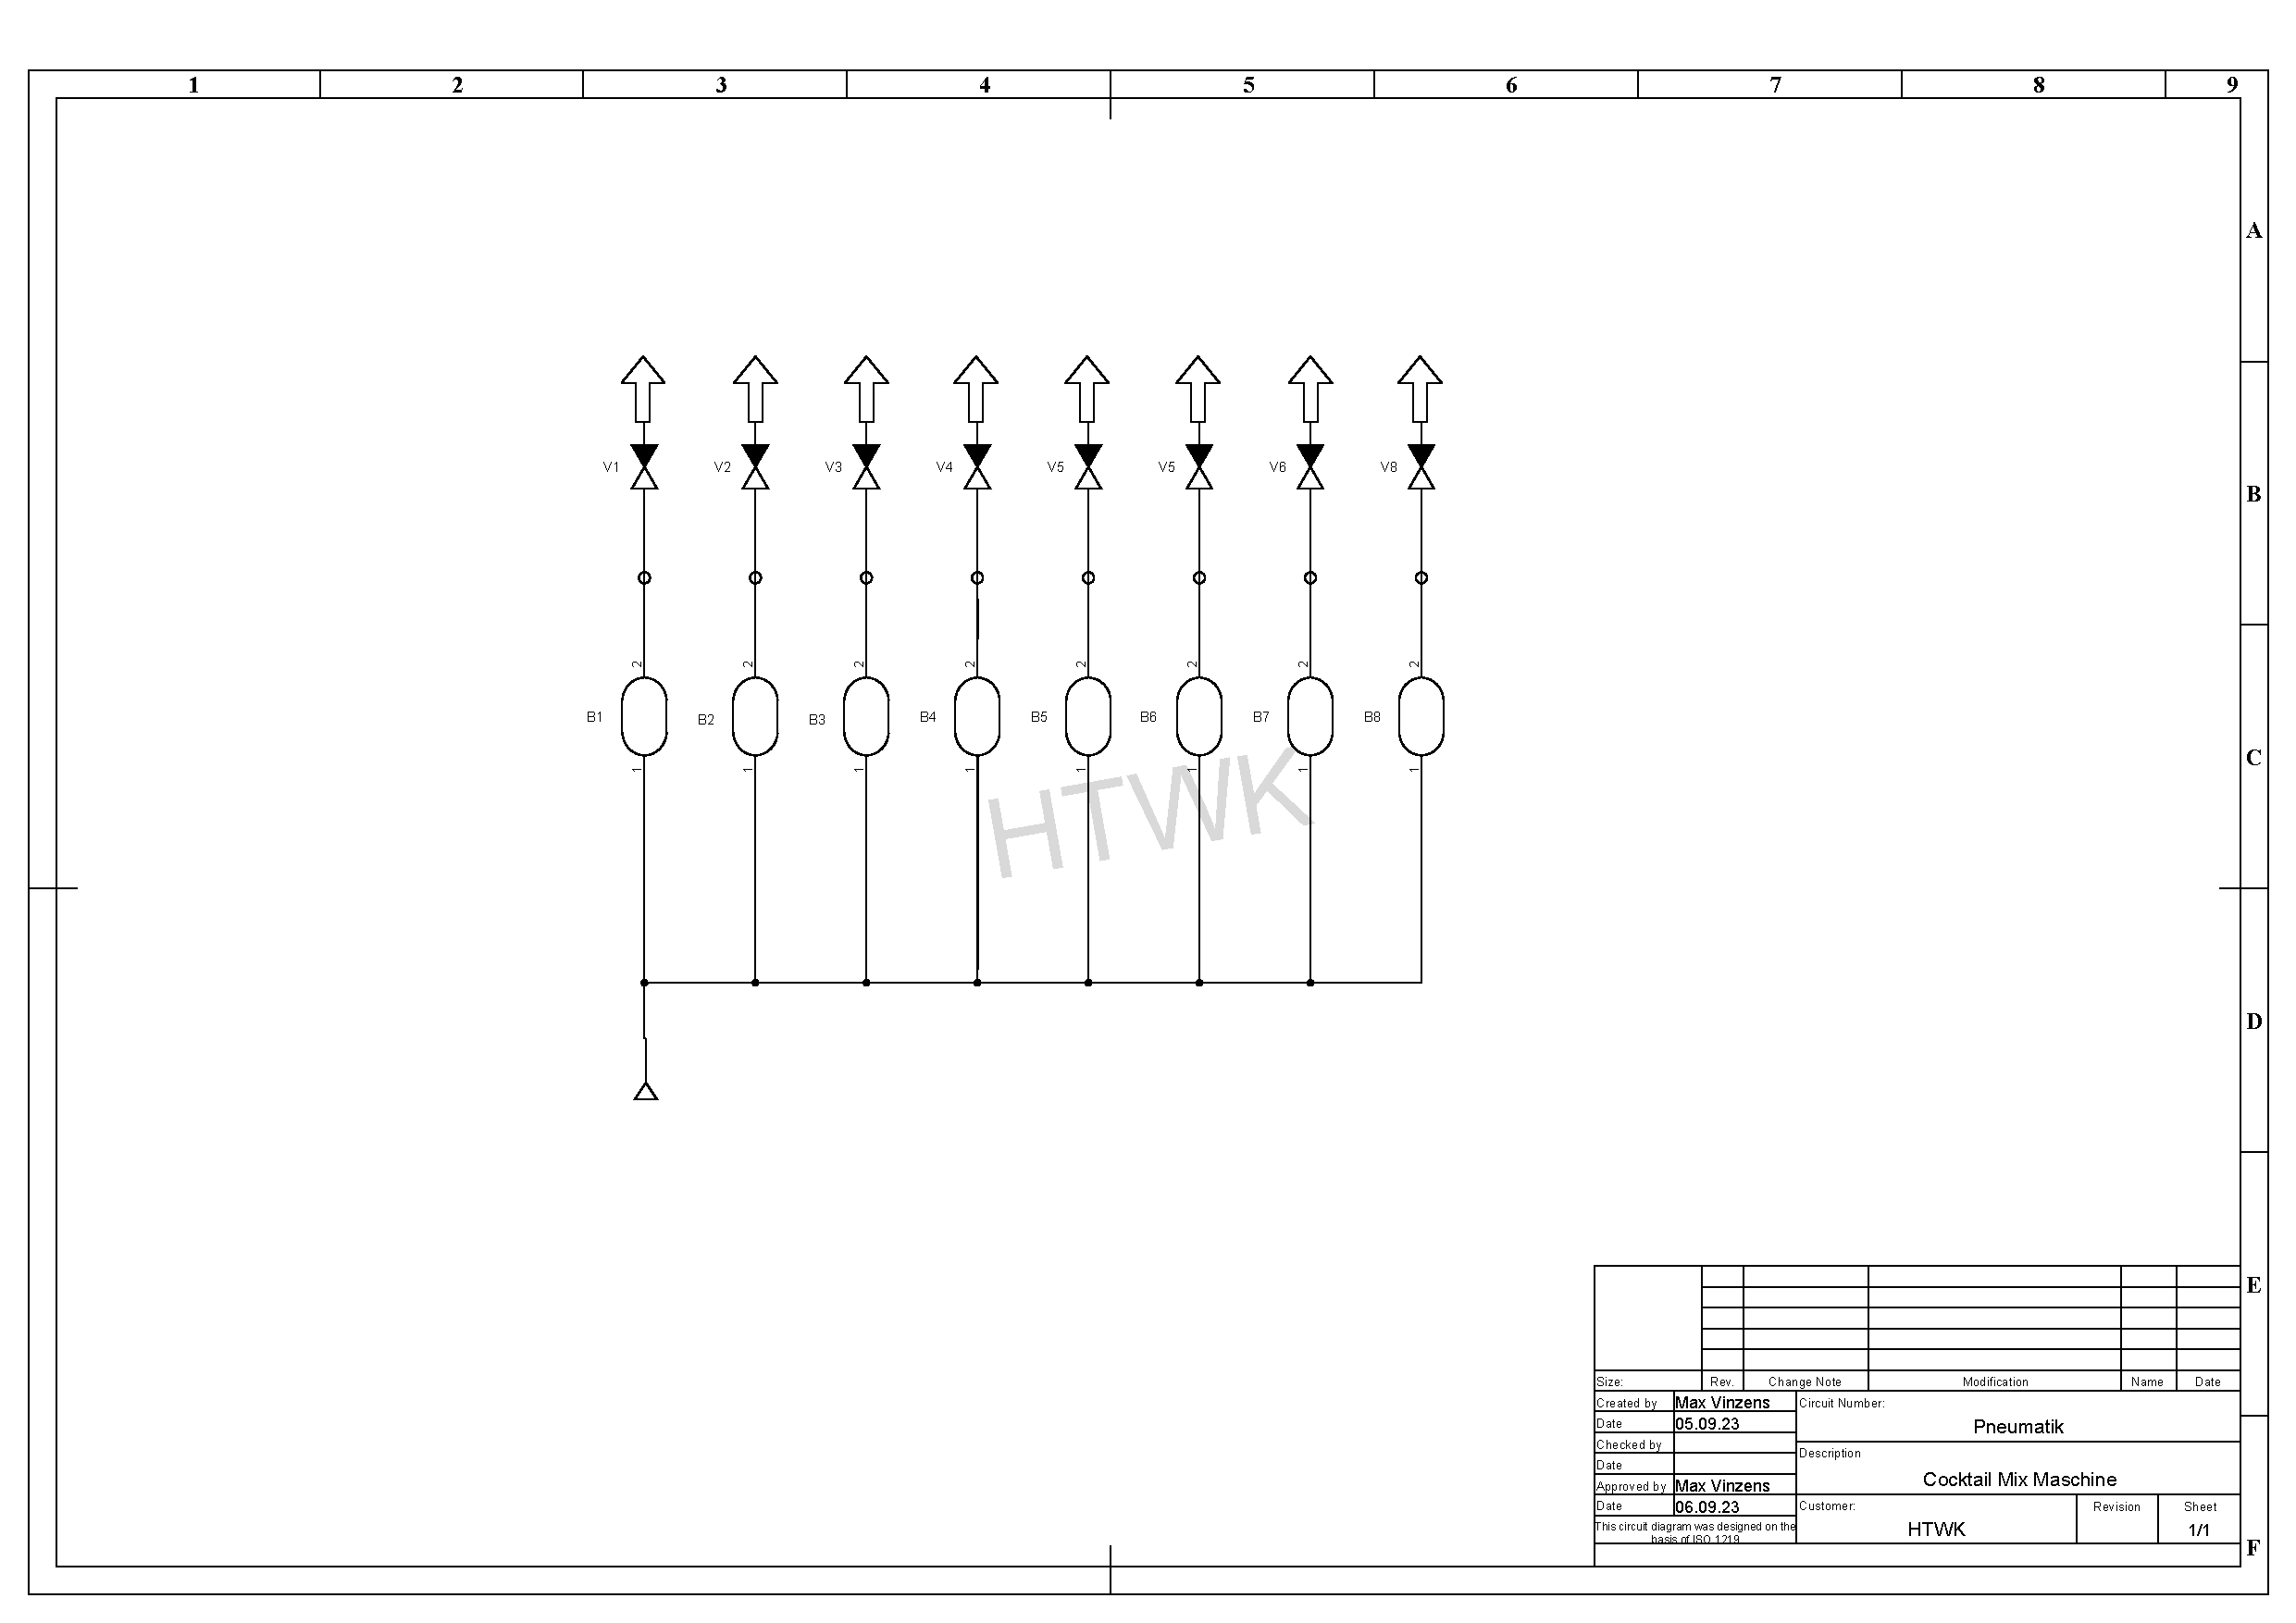
\includegraphics[width=1\textwidth]{Pneumatik (Version2).pdf}
		\centering
		\caption{Pneumatikplan}
	\end{figure}
	
	\chapter{SPS-Programm}
	Bevor ich mit der Programmierung starten konnte, musste ich mich erst auf eine Programmiersprache festlegen. Meine ersten Gedanken gingen in Richtung Ablaufsteuerung mit GRAPHCET, nach der Rücksprache mit unserem Betreuer wurde klar, dass eine textbasierte Sprache verwendet werden soll. Da ich mich sehr gut in C auskenne, habe ich mich für diese Sprache entschieden.\\
	Im nächsten Schritt habe ich eine Moore-Maschine entworfen, jedoch bin ich nach einer Zeit der Programmierung auf Probleme gestoßen. Die SPS kommuniziert nicht direkt mit dem Display, sie stellt einen Webserver zur Verfügung und das Display greift auf diesen zu. Das hat es mir erschwert benötigte Informationen zu gewinnen und auszuwerten.\\
	Um diese Probleme zu umgehen, musste ich einen neuen Automaten entwerfen, er war nicht ganz so elegant aber am Ende hat er funktioniert.\\
	Der Automat hat drei Zustände 1: Grundzustand, 2: Shot und 3: Cocktail. Zwischen diesen Zuständen wird immer hin und her gewechselt, je nachdem wo gerade "Start" gedrückt wurde. In den Grundzustand kommt man immer mit dem Reset-Taster auf dem Display. Der Automat ist in folgender Grafik zu sehen: \\
	
	\begin{figure}[htb]
		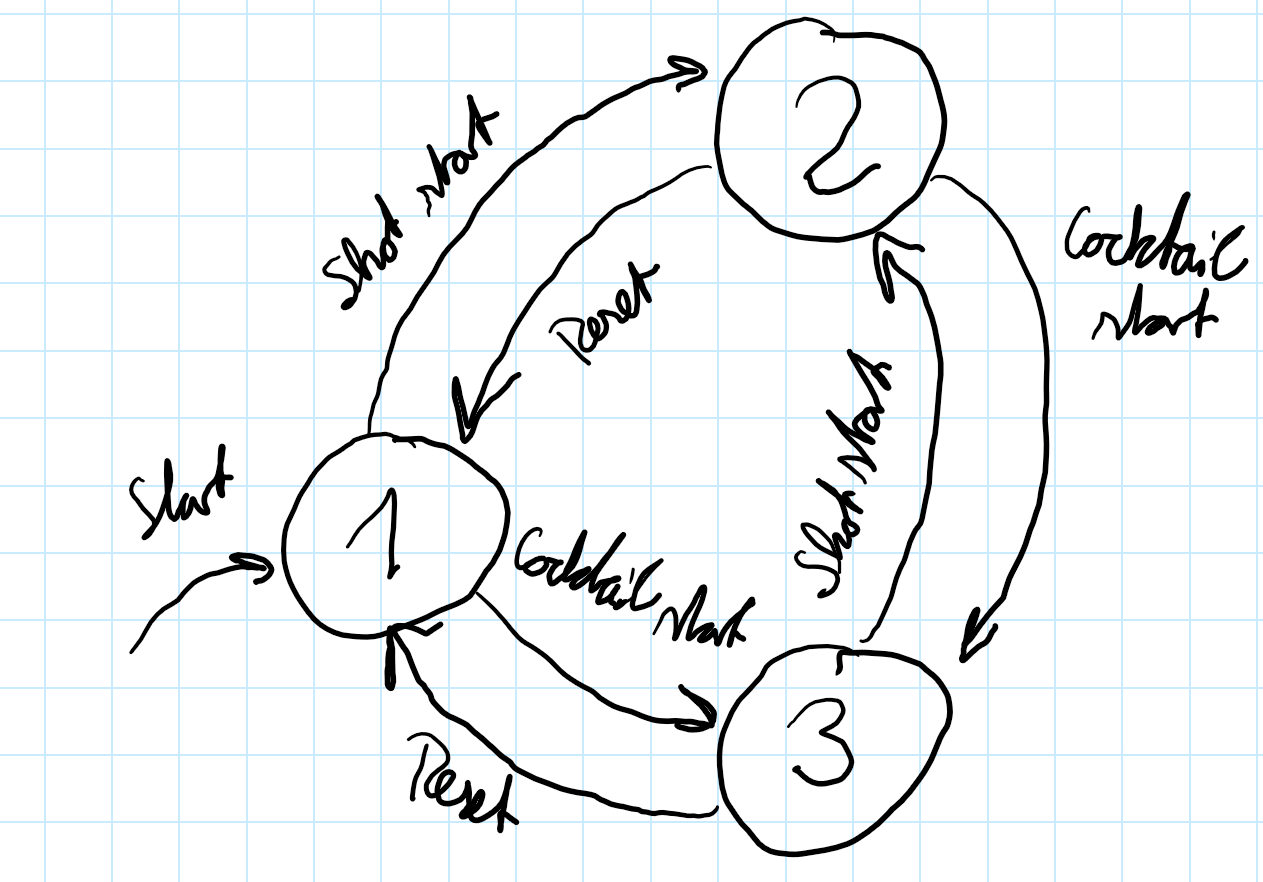
\includegraphics[width=0.65\textwidth]{Leons Zustandsautomat}
		\centering
		\caption{Zustandsautomat}
	\end{figure}
	
	Jetzt war alles klar und ich konnte anfangen das Programm zu schreiben. Um den Code übersichtlicher und besser lesbar zu gestalten, wollte ich mit Prozeduren und Funktionen arbeiten, dies ist mir leider nicht gelungen, da die Entwicklungsumgebung mit eigens erstellten Prozeduren und Funktionen Probleme hatte. Aus diesem Grund blieb mir nicht anderes übrig als die nicht so schöne aber funktionale Lösung zu wählen (den Code immer zu kopieren), was dazu geführt hat, dass das Programm sehr lang wurde.\\
	Ein weiteres Hindernis war, dass ich keine Schleifen verwenden konnte, da die SPS sonst eine Zykluszeitverletzung wirft.\\
	Durch eine if-else-Konstruktion habe ich die einzelnen Zustände implementiert und je nachdem welcher Shot oder welcher Cocktail ausgewählt wurde weiter verschachtelt.\\
	Die Implementierung der Shots war relativ einfach. Bevor der Shot gestartet werden konnte wurden einige sicherheitsrelevante Faktoren abgefragt, wie z.B. dass die Behälter nicht leer sind und das ein Becher in der Maschine steht. Anschließend wird das gewünschte Ventil für den Schnaps geschaltet und bleibt so lange geschaltet bis die Waage einen Gewichtsunterschied von 4 cl registriert. Wird dieser Grenzwert überschritten schaltet die Pumpe und das Ventil ab und die Menge wird aus dem Speicher abgezogen.\\
	Die Implementierung der Cocktails war etwas schwieriger, hier habe ich wie bei den Shots erstmal eine Sicherheitsabfrage durchgeführt, anschließend wurde über eine if-Kostruktion die Größe gesetzt. Anschließend wurde die Kundenentscheidung bezüglich des Eises ausgewertet, falls der Kunde Eis möchte, wird der Motor so lange angesteuert, bis er sich genau eine Runde gedreht hat. Falls nicht wird dieser Prozess übersprungen. Nun beginnt der eigentliche Prozess des Cocktailmischens. Dieser ist mit geschachtelten if-else-Konstruktionen gelöst, bei denen nach und nach Flags für die Zutaten gesetzt werden. So lange eine Zutat nicht fertig ist, wird der if-Zweig durchlaufen in dem der Ausgang gesetzt wird und das Gewicht abgefragt wird. Ist das Sollgewicht erreicht wird das Flag gesetzt und der Else-Zweig durchlaufen der sich wieder in die gleiche if-else-Konstruktion der nächsten Zutat gliedert. Im letzten Durchlauf werden wieder die Füllstände angepasst.\\
	Im unteren Teil des Programms ist der Zustandwechsel realisiert, auch hier sind die Sicherheitsabfragen in die Bedingungen implementiert und natürlich der entsprechende Taster auf dem Display der den Shot oder Cocktail startet.\\
	Der letzte Teil des Programms ist das Reinigungsprogramm, das ist eine Einzelansteuerung der Aktoren. Auf das Einfügen des Programms in die Dokumentation verzichte ich, da das komplette Projekt einschließlich Quellcode im Git hinterlegt ist.\\
	   
	\chapter{3-D Druck}
	
	\section{Eisbehälter}
	
	\subsection{Ausgangsgedanke}
	Da es, wie eingangs schon erwähnt, bereits eine von Studenten der HTWK entwickelte
	Cocktailmaschine gab, war es das Ziel, diese in einer neuen Version zu verbessern. Dabei
	hatten wir uns als Projektgruppe die Anforderung gestellt, dass unser Modell auch die
	Möglichkeit haben soll, auf Wunsch Eis zum Cocktail hinzuzugeben.\\\\
	
	\subsection{Ideenfindung}
	Die Ideenfindung war dabei mit einigen Schwierigkeiten verbunden, da auch eine
	Internetrecherche wenig zu diesem Thema beitragen konnte.
	Unsere ersten Gedanken gingen in Richtung eines Dosierers mit einem Magazin, in dem die
	Eiswürfel gestapelt werden, ähnlich dem Magazin einer Pistole oder dem
	Traubenzuckerspender für Kinder. Die Eiswürfel würden dann durch einen seitlichen Stempel
	herausgedrückt.
	Eine zweite Variante fiel Benjamin ein, als er an einem Haus vorbei ging, an dem früher ein
	Kaugummiautomat hing. Ein solcher war mit Kaugummikugeln und/oder Kugeln mit kleinem
	Spielzeug gefüllt. Man steckt eine Münze in den dafür vorgesehenen Schlitz und dreht einen
	Griff um 180°: Die Kugel fällt unten heraus.
	Diese Technik, in ähnlicher Form, für den Eisdosierer zu verwenden, gefiel uns besser, da
	hiermit dann auch Crashed Ice verwendet werden kann.
	So fing Benjamin, als Hauptverantwortlicher für das Design des Eisdosierers, an, diese Idee
	umzusetzen. \\\\
	
	\subsection{Grundüberlegung}
	Da wir, wie schon beschrieben, nicht zuerst die innen liegende Technik entwickelten und folgend
	das Gehäuse, sondern die Größe des Gehäuses bereits definiert war, musste Benjamin als
	erstes klären, wie viel Platz ihm für den Eisdosierer im Gehäuse zur Verfügung steht und an
	welcher Stelle der Cocktailbecher platziert werden soll. Wie der Zeichnung zu entnehmen ist,
	stand der gesamte Raum oberhalb der geplanten Cocktailbecheroberkante zur Verfügung (im
	unteren Bereich finden dann Ventile, Schläuche e.t.c. Platz). (Die genauen Abmaße aller
	Bestandteile sind bitte ebenfalls der Zeichnung zu entnehmen, um den Lesefluss nicht zu
	erschweren.)
	Hier mussten alle notwendigen Elemente, entsprechend des technischen Prinzips des
	Kaugummiautomaten, platziert werden:\\ \\
	– der Aufbewahrungsbehälter des Eises, der im unteren Bereich, zum Auslass hin,
	trichterförmig zuläuft (um das Rutschen des Eises zu ermöglichen)\\ \\
	– die Dosiereinheit, bestehend aus einer Dosierwalze, welche in einem offenen Dosierfach
	eine fixe Menge Eis aufnimmt und dieses während einer Drehung um insgesamt 360° in
	den darunterliegenden Ausgangstrichter auswirft, sowie zusätzlich einem Motor mit
	zusätzlichem Kegelgetriebe, welcher die Drehung der Walze übernimmt\\ \\
	– der Ausgangstrichter, in den auch alle weiteren Zutaten eingeleitet werden und der diese
	Zutaten in den Cocktailbecher füllt.\\ \\
	\newpage
	Als Material wurden für die selbst entwickelten Teile PLA und PETG gewählt, um das Projekt mit
	Hilfe von 3D-Druck umsetzen zu können. Im Verlauf wurden also die benötigten Teile mit Hilfe
	eines Programms entwickelt und zum Druck weitergeleitet.
	Bei beiden oben genannten Materialien ist die Lebensmittelechtheit gegeben. Für einen
	professionellen Einsatz, wäre als Material möglicherweise Edelstahl zu bevorzugen. In diesem
	Fall müsste gegebenenfalls über eine zusätzliche Isolierung des Eisbehälters nachgedacht
	werden.
	Eine Dämmung wurde für unseren Eisbehälter/unsere Cocktailmaschine nicht eingeplant, da
	davon ausgegangen werden kann, dass im Betrieb auf Veranstaltungen das Eis rasch genug
	
	verbraucht wird, so dass eine zusätzliche Dämmung als nicht notwendig erachtet wird. Diese
	ließe sich aber jederzeit, bei Bedarf, ergänzen.\\\\
	
	\subsection{Das Kernstück: die Dosiereinheit}
	Das Kernstück ist die eigentliche Dosiereinheit mit der Dosierwalze (und Gehäuse).
	Wie folgt soll diese funktionieren: Wird über das Bedienfeld bei der Cocktailauswahl die Option
	„Eis hinzufügen“ gewählt, wird ein Motor angesteuert, der die Dosierwalze um 360° dreht. Damit
	bewegt sich das Eis-Dosierfach der Walze nach unten und entlässt im Verlauf der Drehung das
	darin befindliche Eis in den Ausgangstrichter, welches darin weiter bis in den Cocktailbecher
	rutscht.
	Pro Cocktail soll eine bestimmte Menge Crushed Ice oder Eiswürfel, in den Cocktailbecher
	dosiert werden. Daraus definiert sich die Größe des Eis-Aufnahmefaches in der Dosierwalze –
	und daraus folgend, die Gesamtgröße der Dosiereinheit.
	Daher musste diese zuerst in Größe und Ausführung geplant werden. Der übrige verfügbare
	Platz steht dann dem Eisbehälter sowie dem Ausgangstrichter zur Verfügung.
	Die Dosiereinheit (Gehäuse mit der Dosierwalze) ist direkt an dem oberhalb befindlichen
	trichterförmigen Auslass des Eis-Aufbewahrungsbehälters befestigt und verschließt diesen mit
	der Walze daher auch automatisch. Im Ausgangszustand befindet sich das Eis-Dosierfach der
	Walze oben am Auslass des Behälters, so dass das Eis in dieses fallen kann. Das Dosierfach
	erstreckt sich über die gesamte Länge der Walze. Über zusätzliche Einlegeteile kann/könnte
	gegebenenfalls bei Bedarf die Menge der Eisportionen verringert werden.
	An die Walze wurde ein Motor verbaut, welcher diese antreibt. Im Sammelsurium unseres
	Laborleiters fand sich ein passender Motor mit Getriebe (passende Größe und passende
	sonstige Werte, wie Drehmoment und Spannung).
	Für eine Platzierung des Motors im 90°-Winkel zur Walze wurden zwei Kegelzahnräder
	entwickelt, die zudem durch ihre Übersetzung (15 Zähne und 35 Zähne, letzteres im
	Durchmesser passend zur Seitenfläche des Gehäuses der Dosiereinheit) die Geschwindigkeit
	nach dem Motorgetriebe nochmals reduziert.
	Der Motor wird über die Steuereinheit angesteuert. Dafür wurden zwei Endlagenschalter (mittels
	gefertigter Halterung) am Dosierer befestigt und zudem am großen Zahnrad eine Schraube als
	Auslöser der Endlagenschalter. Somit erkennt die Steuereinheit, wenn die Dosierwalze die
	gewünschte Umdrehung um 360° vollendet hat und stoppt den Motor.
	(Erklärung zu den zwei Endlagenschaltern: Schalter 1: ist ausgelöst, wenn sich die Walze in der
	Ausgangsposition befindet – Schraube auf Schalter. Läuft die Walze an, bewegt sich die
	Schraube weg - Schalter 1 schaltet aus. Im Verlauf löst die Schraube den Schalter 2 aus. Das
	ist eine programmiertechnische Vereinfachung, um der Steuereinheit das Signal zu geben, dass
	sich die Walze in Bewegung befindet und sie nun darauf achten soll, wann Schalter 1 wieder
	ausgelöst wird, also die Walze sich wieder in der Ausgangsposition befindet.)\\ \\
	
	\subsection{Eis-Aufbewahrungsbehälter und Ausgangstrichter}
	Nachdem nun die Größe der Dosiereinheit feststand, wurde das passende Maß für den Ausgangstrichter festgelegt. Folgend definierte sich daraus der verfügbare Platz für den Eis-Aufbewahrungsbehälter inklusive trichterförmigem Auslass und damit dessen maximale Größe. Diese wurde ausgenutzt.
	Der Trichter im Behälter sorgt dafür, dass das im Behälter befindliche Eis, auch bis zum Rest, in die Dosierwalze rutschen kann.\\ \\
	\newpage
	
	\subsection{Aufgetretene Probleme und Fehler}
	Als die fertigen Teile aus dem Druck kamen, fiel Benjamin auf, dass er offensichtlich die
	Toleranzen nicht entsprechend beachtet hatte und daher an etlichen Stellen nachgearbeitet
	werden musste. So passte die Dosierwalze nicht richtig in das Dosiergehäuse. Um sie
	gleichmäßig etwas zu verschlanken, drehte er sie per Drehbank nochmal etwas ab.
	Ebenso musste die Aufnahme des großen Zahnrades etwas angepasst werden.
	Die ersten „Trockentestes“ verliefen problemlos. Als wir dann aber mit Crashed Ice testeten,
	verklemmte sich dieses zwischen Dosierwalze und Gehäuse und das kleine Zahnrad blieb
	stehen, während die Motorwelle in der Aufnahme des Zahnrades durchdrehte. Dieses Problem
	konnte durch Festkleben des kleinen Zahnrades auf der Motorwelle sowie durch eine
	zusätzliche, überlappende Schräge in der Öffnung des Eistrichters zum Dosierbehälter
	behoben werden.
	Ein letztes Problem trat im Übergang des Ausgangstrichters zum Cocktailbecher auf. Hier
	schossen das Eis sowie die anderen Cocktailzutaten teilweise über ihr Ziel, den Cocktailbecher
	hinaus, landeten also nicht ordnungsgemäß in diesem. Hier brachte ein Spritzschutz am
	Ausgangstrichter einfache Abhilfe, gegen den nun die Zutaten (vor allem das Eis) prallen und
	damit spritzfrei in den Becher gelangen können.\\ \\
	
	\section{Bildschirmhalterung}	
	Um dem Nutzer ein möglichst angenehmes Bedienen zu ermöglichen, soll der Bildschirm, über dem man die Cocktails und Shots auswählen kann in einer Halterung befestigt werden. Dafür wurde mittels 3D-Druck eine solche Halterung entwickelt. Der Bildschirm soll dabei so positioniert werden, dass der Nutzer, wenn er vor der Cocktailmaschine steht, bequem auf diesen schauen kann. Daher wurde die Halterung so entwickelt, dass der Bilschirm in einem 30 Grad Winkel zum Untergrund steht.
	Der Bildschirm soll dabei so positioniert werden, dass der Nutzer, wenn er vor der Cocktailmaschine steht, bequem auf diesen schauen kann. Daher wurde die Halterung so entwickelt, dass der Bilschirm in einem 30 Grad Winkel zum Untergrund steht. Die eine Seite der Halterung ist offen und hat einen seperaten Deckel, um sie zu schließen. Dieser Deckel hat ein Loch in einer hinteren Ecke, durch welches die Kabel zum Anschließen des Bildschirms verlegt werden. Der Bildschirm selber wird von vorne in die Halterung reingelegt. 
	Auf diese Weise schließt der Bildschirm bündig an die Halterung an und alle ausgehenden Kabel werden sauber hinausgeführt.\\
	\begin{figure}[htb]
		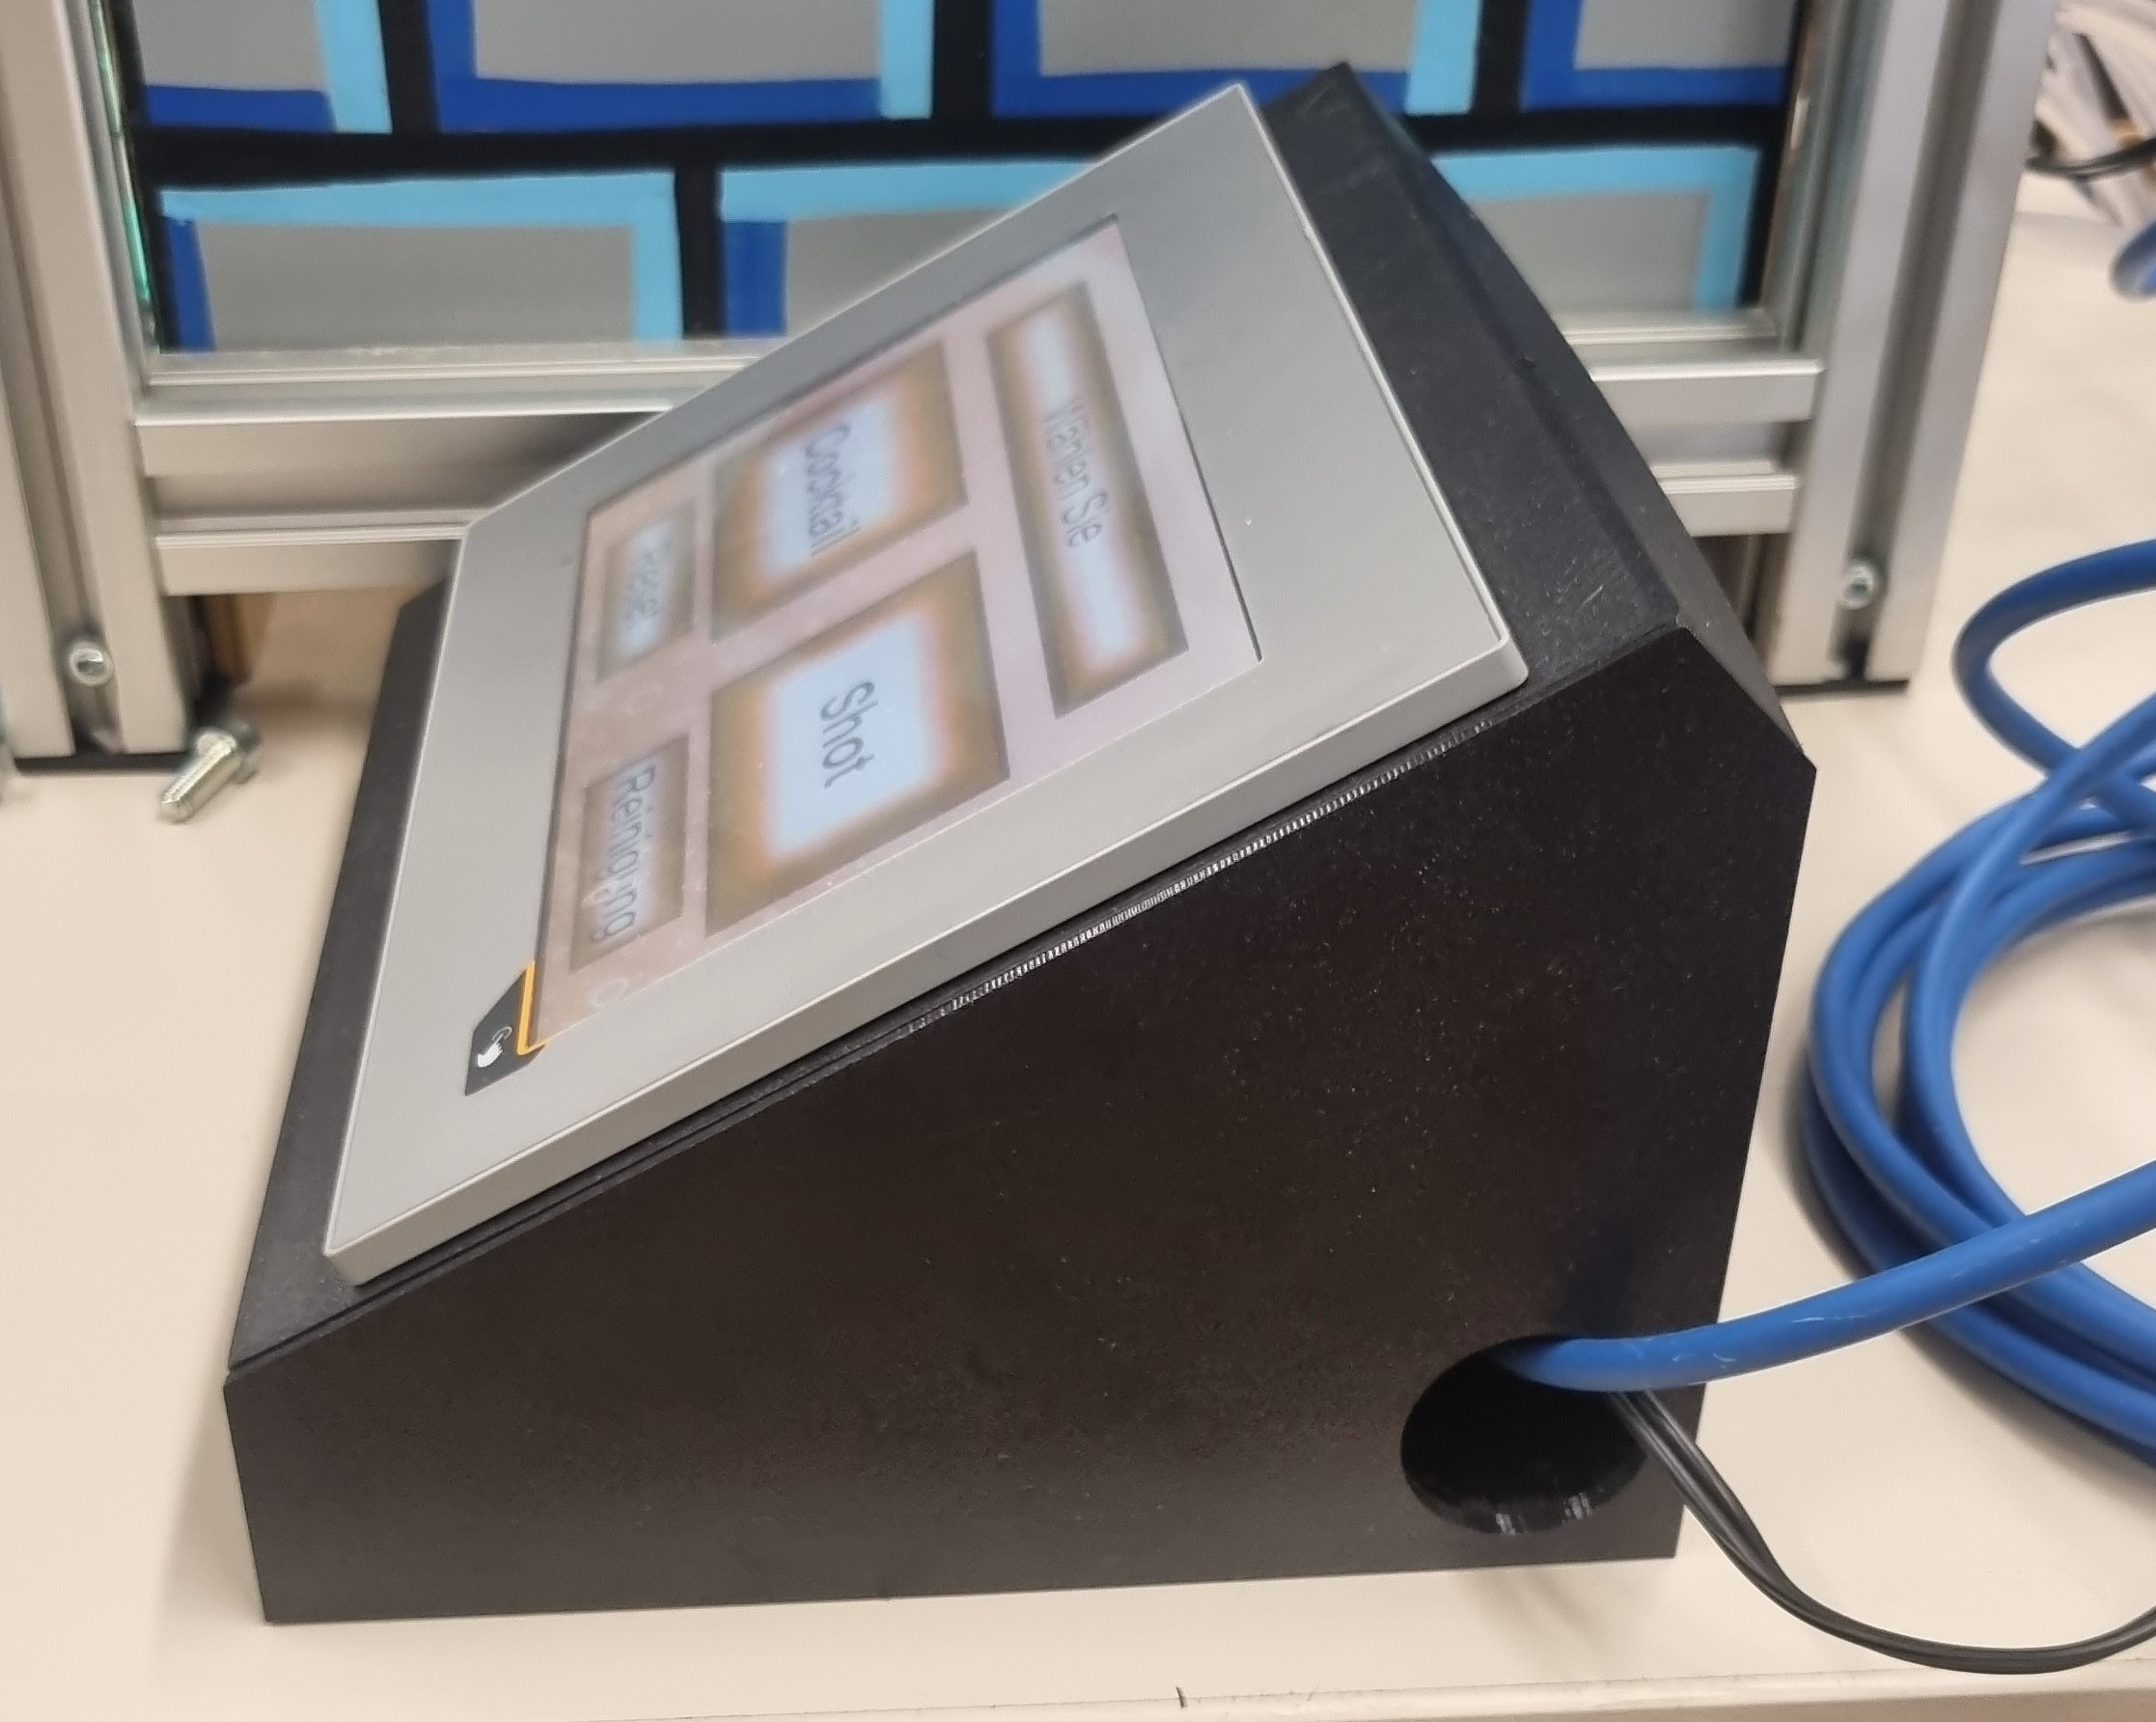
\includegraphics[width=0.5\textwidth]{Abb.2_Bildschirmhalterung_komplett}
		\centering
		\caption{Bildschirmhalterung}
	\end{figure}
	
	\section{Verkleidung der Öffnung}
	Die Öffnung, durch welche der Trinkbecher in die Maschine gestellt werden soll, wurde aus dem Holz herausgesägt. Da die Form händisch ausgeschnitten wurde, sind gerade und gebogene Linien nicht ganz sauber. Zudem sind nun die Ränder der Öffnung etwas scharfkantig. Daher haben wir uns für eine Verkleidung der Öffnung entschieden, die mittels 3D-Druck gefertigt werden soll. Die U-förmige Figur kann einfach auf die Öffnung gelegt und festgeklebt werden. In Abbildung 9.2 sieht man die fertige Verkleidung.
	
	\begin{figure}[htb]
		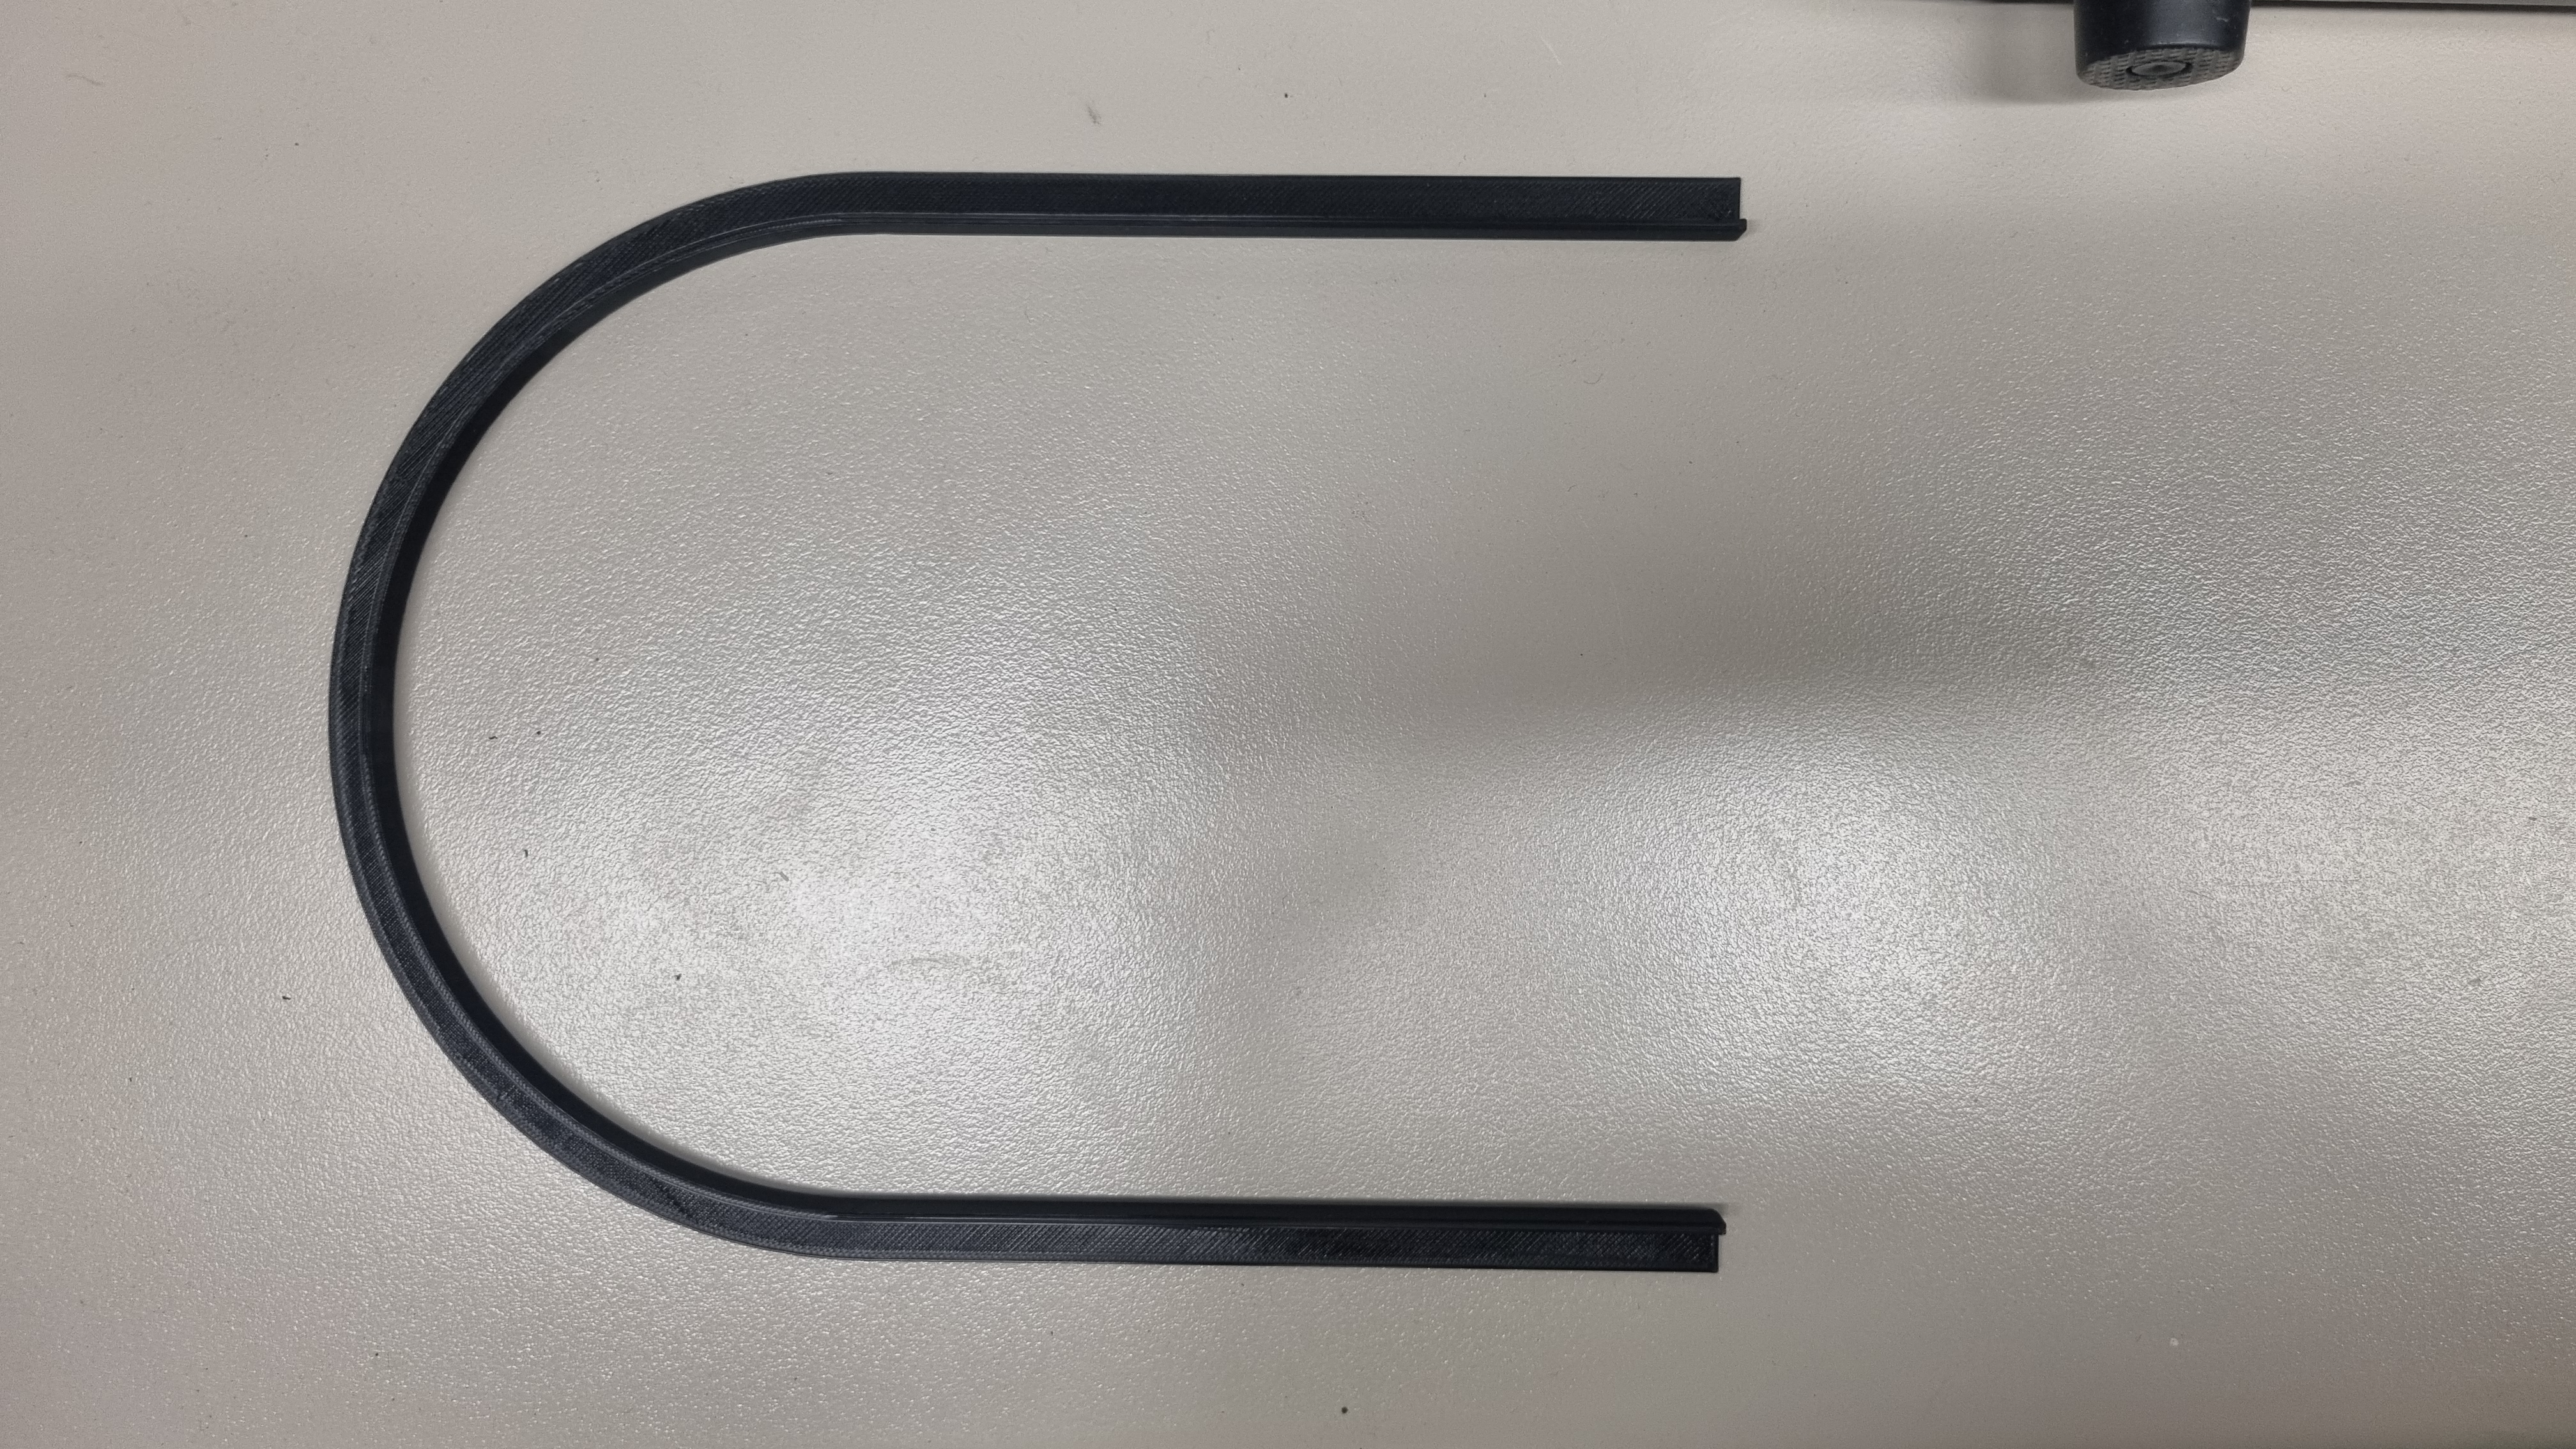
\includegraphics[width=0.5\textwidth]{Abb.4_Verkleidung}
		\centering
		\caption{Türbogen}
	\end{figure}
	
	\section{Becherständer}
	Damit der Becher in die Cocktailmaschine gestellt werden kann, benötigen wir einen Ständer. Dieser muss an die Wägezelle angebracht werden, sodass stets das Gewicht der Flüssigkeit im Becher gemessen werden kann. Die Wägezelle hat eine vorgefertigte Bohrung für eine M4-Schraube. Daher steht fest, dass der Ständer in der Mitte eine Öffnung für eine solche Schraube bieten muss. Da der Becher, eine runde Form hat, wurde sich auch für einen runden Ständer entschieden. Auf Basis dieser Fakten wurde folgender Becherständer für den 3D-Druck entworfen.
	
	\section{Becherhalterung}
	Im Laufe der Tests haben wir festgestellt, dass gerade beim Einschütten von Eis der Becher sehr schnell umkippt. Um dem entgegen zu wirken muss eine Becherhalterung entwickelt werden, die den Getränkebecher an Ort und Stelle hält. Eine solche Halterung wurde mittels 3D-Druck hergestellt. Die Konstruktion soll rund sein und auf vier Balken getragen werden, welche an dem Becherständer festgeklebt werden können. Leider wurde bei dieser Konstruktion nicht bedacht, dass der Becher im vollen Zustand nicht mehr aus der Halterung entnommen werden kann, ohne jegliche Flüssigkeit auszuschütten. Daher wurde die Halterung kurzerhand abgeändert. Der Runde Kreis zum Halten wurde mit einer Zange fast halbiert, sodass gerade so noch drei der vier Beine dran sind. Dadurch hat die Halterung eine Klemmfunktion entwickelt, die ausreichend zum Halten des Bechers ist (siehe Abbildung 9.3).\\

	\begin{figure}[htb]
		\includegraphics[width=0.5\textwidth]{Abb.7_Becherhalterung_und_Becherständer}
		\centering
		\caption{Halterung}
	\end{figure}
	
	\chapter{Gestaltung}
	
	\section{Layouts}
	Damit die Cocktailmaschine benutzerfreundlich ist, muss für jeden Anwender klar und deutlich zu erkennen sein, wie er die Maschine bedienen muss, um am Ende ein Getränk zu erhalten. Um dem gerecht zu werden wurde sich eine einfache Bedienung über ein Touchpanel gewünscht. Dort soll der Anwender über Buttons entscheiden können, ob er sich einen Cocktail oder einen Shot wünscht (siehe Abbildung 10.1). Auch die Größe eines Cocktails oder ob Eis hinzugefügt werden soll, ist über dieses Panel zu entscheiden und auch ein Abbruch- und Startbutton sollen vorhanden sein (siehe Abbildung 10.1). 
	Damit die Bedienung möglichst einfach ist, haben wir mit möglichst großen Buttons gearbeitet (siehe Abbildung 10.1), die wenig Text oder sogar nur Zeichen beinhalten. Bei der Farbwahl wurde darauf geachtet, eine angenehme Farbe zu wählen, die nicht ins Auge sticht, aber trotzdem guten Kontrast zur Schrift bietet. Dabei haben wir uns für Orange- und Weißtöne entschieden. Diese passen auch zu den größtenteils orangefarbenen Cocktails. Da der Abbruch und der Start von etwas größerer Bedeutung sind, sollten die dafür vorgesehenen Buttons hervorgehoben werden. Daher ist Start grün und Exit rot. Um die Bedienung auch bei der anschließenden Reinigung der Maschine zu vereinfachen, wurde auch hier das Touchpanel eingebunden. Über einen Button auf der Startseite kommt man ins Reinigungsmenü. Hier können alle Ventile und der Motor einzeln angesteuert werden (siehe Abbildung 10.1).
	
	\begin{figure}[htb]
		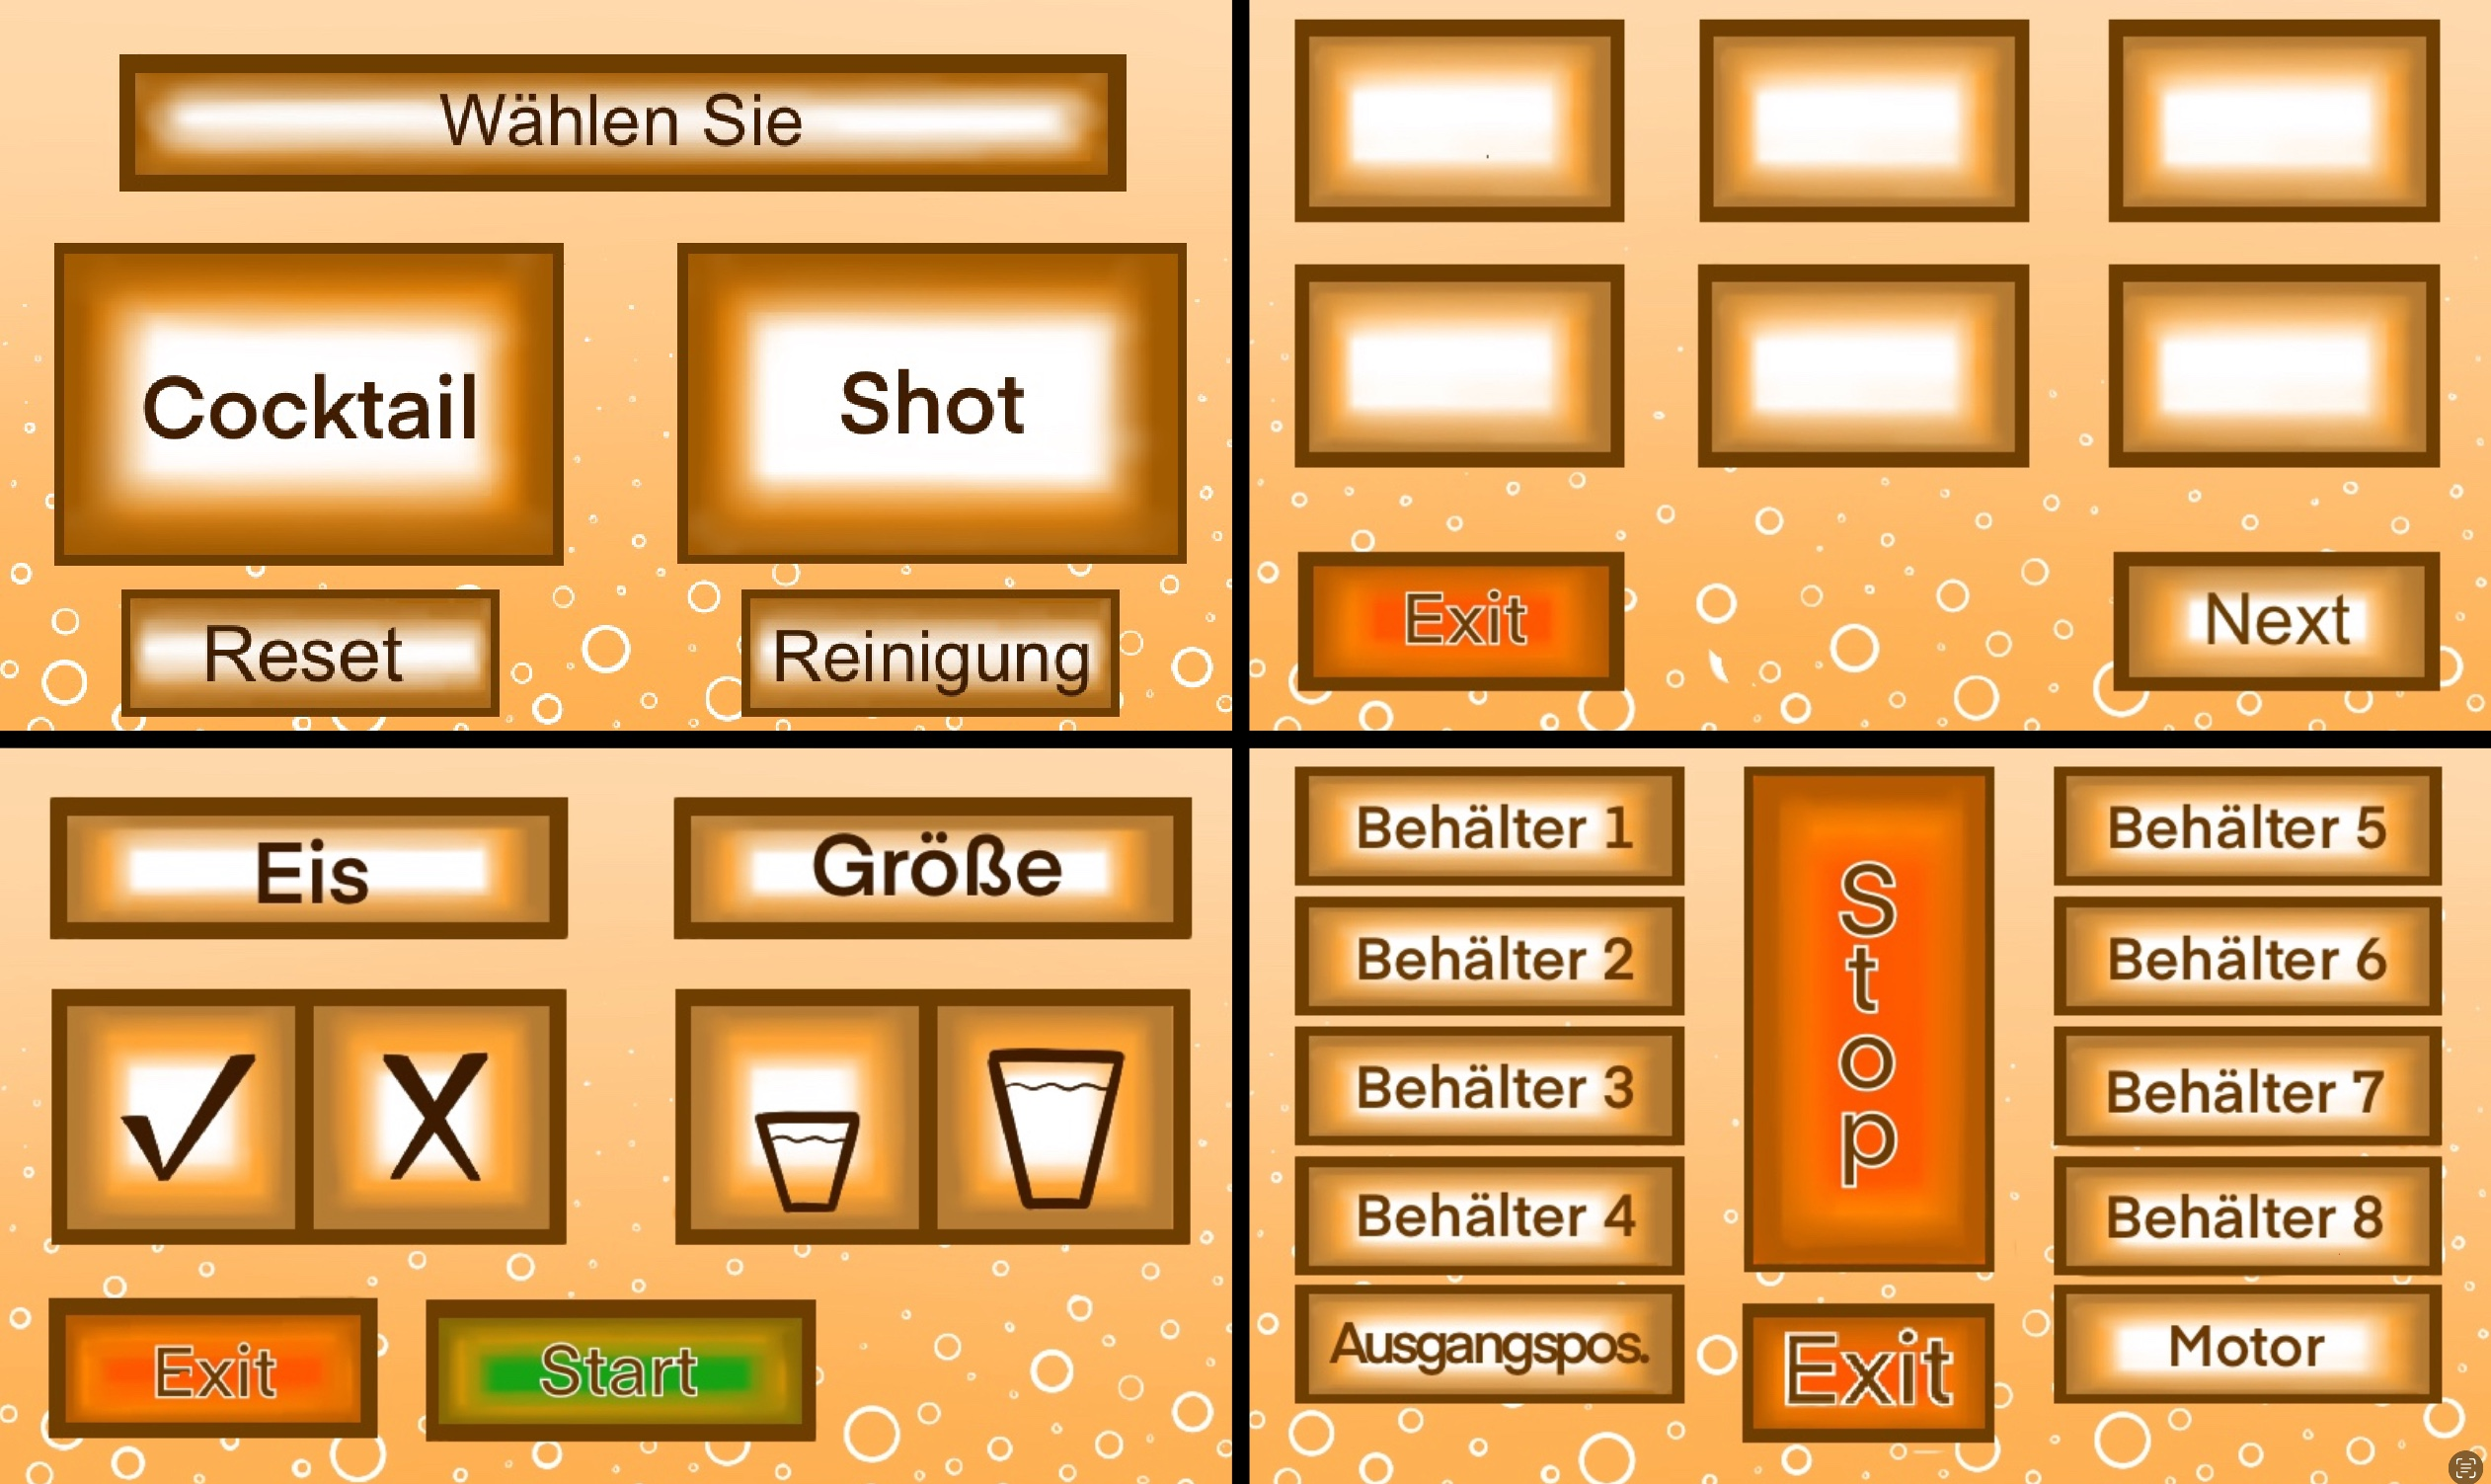
\includegraphics[width=1\textwidth]{Abb.A_Bildschirmpanels}
		\centering
		\caption{Displayanzeigen}
	\end{figure}
	\newpage
	\section{Außenwandgestaltung}
	Damit die Cocktailmaschine von außen ansprechend aussieht und Aufmerksamkeit auf sich zieht, müssen alle hölzernen Außenwände gestaltet werden. Dabei haben wir an eine Art „Industrial Look“ gedacht. Die Maschine sollte im Grundton schlicht sein, aber durch farbige Elemente herausstechen. Ein grauer Unterton mit blauen Aktzenten entsprach dabei am ehesten den Vorstellungen. Die fertigen Wände sind in Abbildung 10.2 zu sehen.\\
	
	\begin{figure}[htb]
		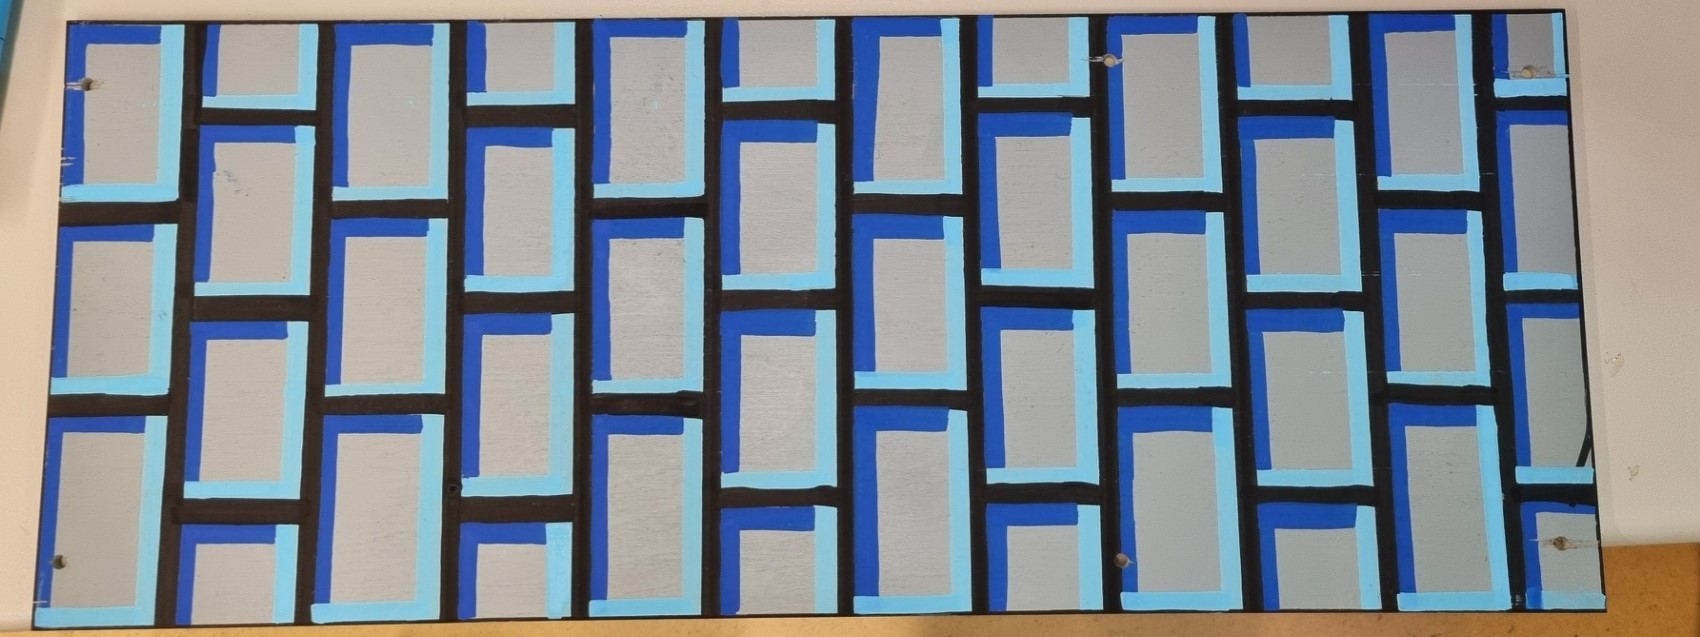
\includegraphics[width=1\textwidth]{Abb.16_bemalte_Holzwand}
		\centering
		\caption{Außenwand}
	\end{figure}
	
	Um dem ganzen einen letzten Effekt zu geben, wird die vordere Außenwand während des Mischvorgangs beleuchtet. Dafür wurden zwei LED-Leisten an die Profilschienen geklebt. Solange ein Cocktail gemixt wird, leuchten diese rot, sobald er fertig ist, leuchtet sie grün (siehe Abbildung 10.3).\\
	
	\begin{figure}[htb]
		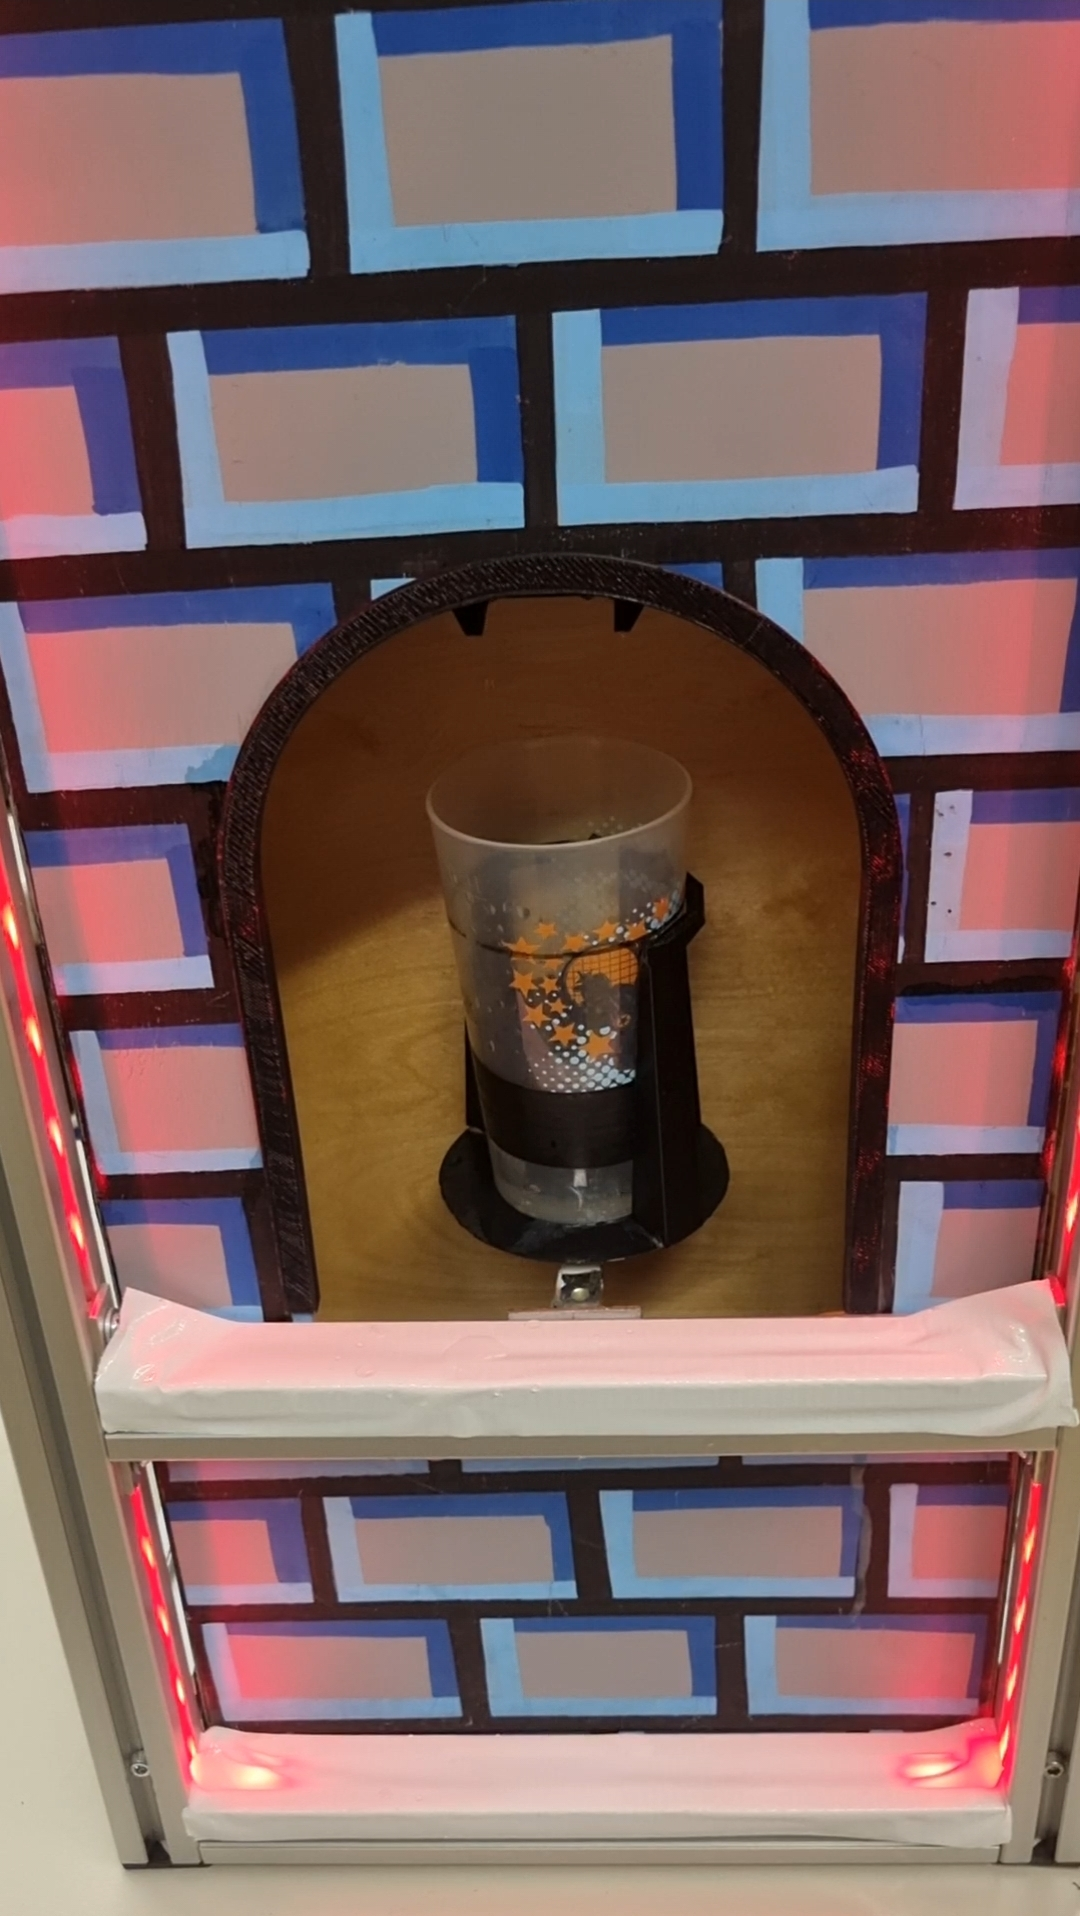
\includegraphics[width=0.4\textwidth]{Abb.17_LED_Beleuchtung}
		\centering
		\caption{Vorderseite}
	\end{figure}	
	
	\chapter{Cocktailauswahl}
	Anfangs haben wir uns um die 50 Cocktails herausgesucht, die mit 8 Zutaten gemischt werden konnten. Diese wurden auch im Programm vorerst mit Dummygewichten hinterlegt. Nachdem wir diese jedoch probiert hatten, entsprachen sie nicht unseren Vorstellungen. Deshalb haben wir sie angepasst und folgende Cocktails sind dabei herausgekommen: \\
	Cocktail 1 ist 3 cl Tequila, 3 cl Rum, 16 cl Orangensaft und 2 cl Zitronensaft \\
	Cocktail 2 ist 5 cl Gin, 18 cl Tonic Water und 2 cl Zitronensaft\\
	Cocktail 3 ist 4 cl Rum, 2 cl Zitronensaft, 13 cl Ananassaft und 5 cl Tonic Water \\
	Cocktail 4 ist 2 cl Vodka, 12 cl Orangensaft, 9 cl Ananassaft und 2 cl Tequila \\
	In der weiteren Cocktailauswahl gibt es den zufälligen Cocktail, hier wird aus denen zur Auswahl stehenden Cocktails einer ausgewählt. Als Krönung gibt es aber noch den richtig zufälligen Cocktail, hier wird ein Cocktail, bestehend aus 4 Zutaten aus den 8 zur Verfügung stehenden Zutaten zusammen gemischt.\\
	Neben der Cocktailauswahl gibt es auch noch eine Auswahl an Shots, diese sind alle 4 cl groß und sind die zur Verfügung stehenden Schnäpse.\\  
	
	\chapter{Reinigung}
	Dadurch das wir unterschiedlichen Flüssigkeiten in den Schläuchen, Ventile und den Behälter
	haben, die verderben können, mussten wir eine Lösung finden.\\\\
	Wir erarbeiteten ein Reinigungskonzept im Stil von GRAFCET.\\\\
	Als Erstes machten wir uns am Anfang eine Vorüberlegung.
	Durch das erstmalige Erproben der Cocktailmaschine und dessen Reinigung, fanden wir Fehler und
	Verbesserungen, sodass wir am Ende ein einfaches und gründliches Reinigungskonzept hatten.
	Wir haben dieses Reinigungskonzept noch einmal in einem dry run mit einer außenstehenden
	Person durchgeführt und aus dessen Fehlern und Verbesserungsvorschlägen das Reinigungskonzept
	verbessert.
	\begin{figure}[htb]
		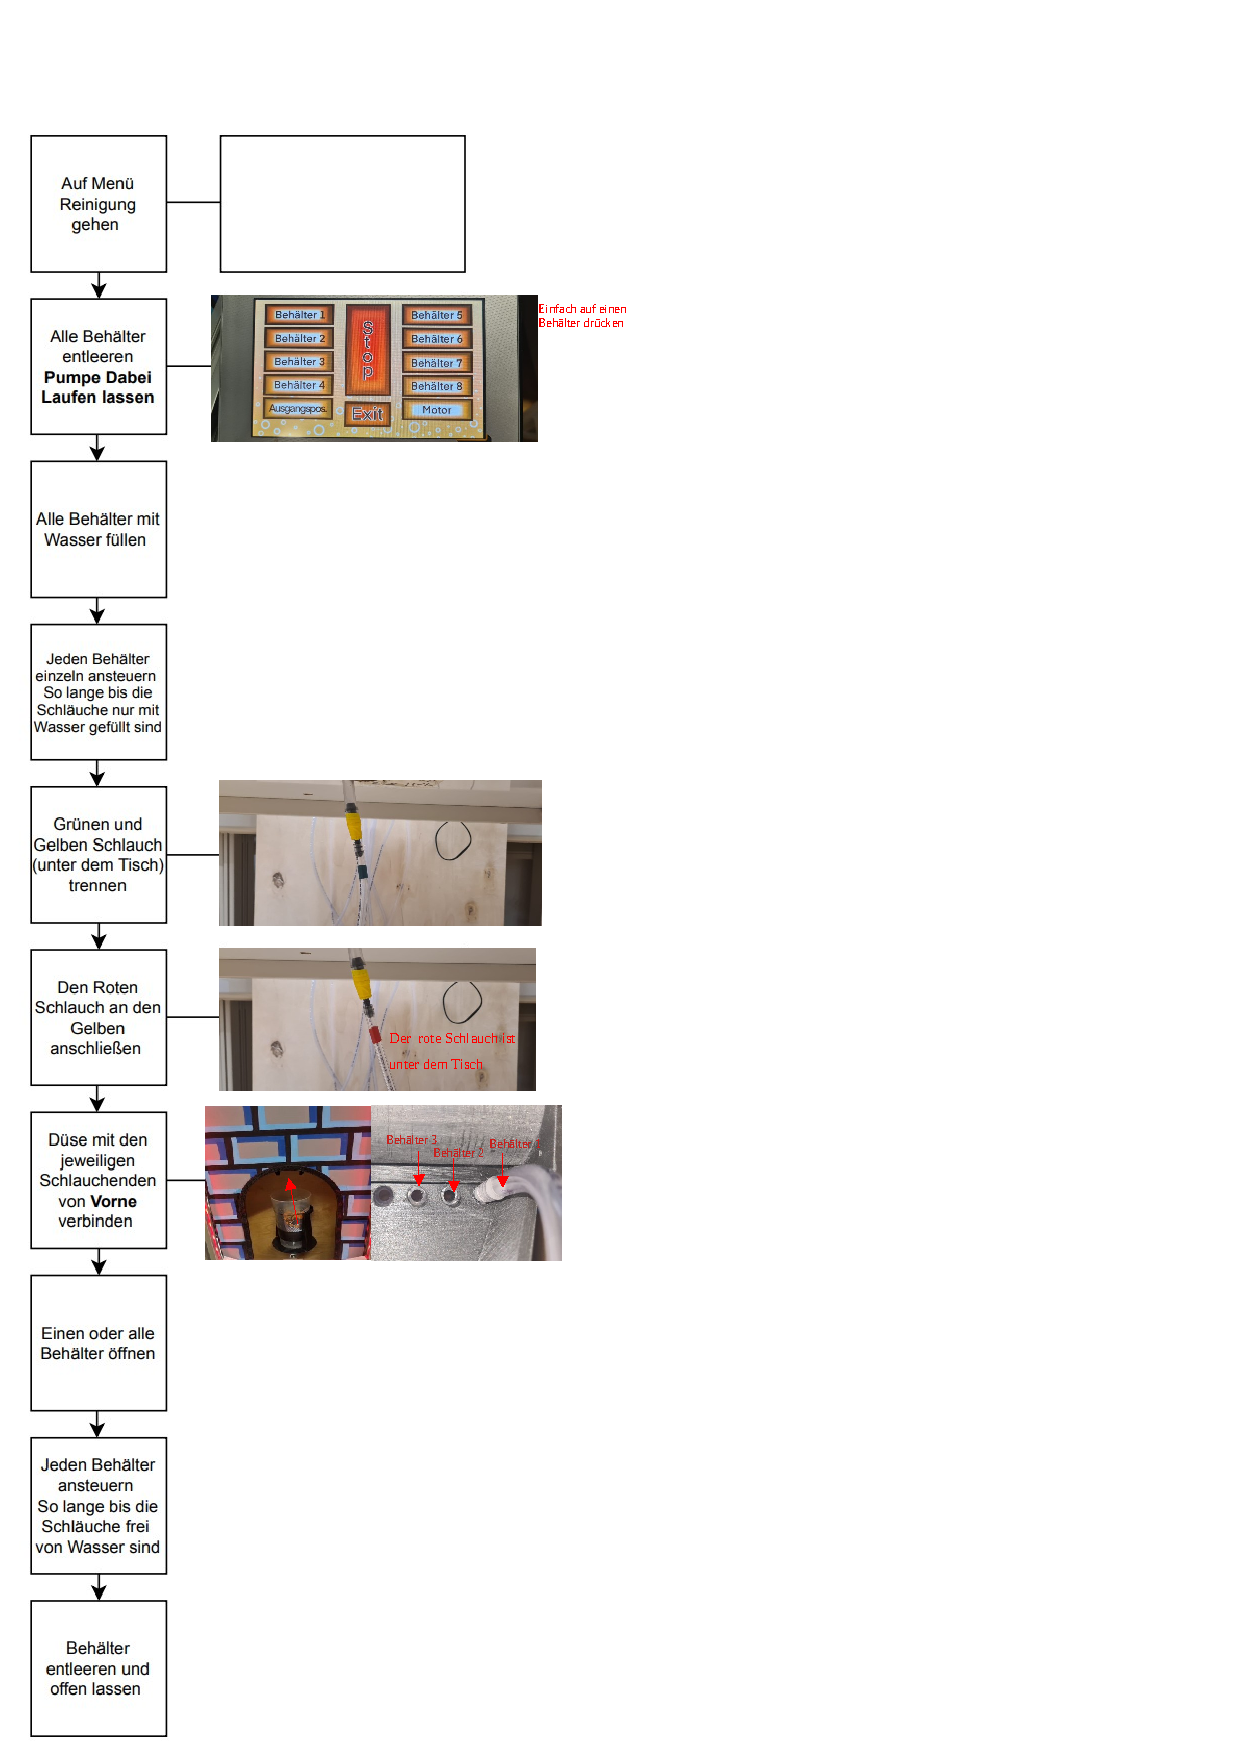
\includegraphics[width=0.65\textwidth]{Sauber zauber.pdf}
		\centering
		\caption{Reinigungsablauf}
	\end{figure} 
	
\end{document}